\documentclass{article}


\usepackage[fleqn]{amsmath}
\usepackage{graphicx}
\usepackage{color}
\usepackage{xspace}
\usepackage{cite}
\usepackage[margin=1in]{geometry}
\usepackage{amsfonts}
\usepackage{array,multirow}
\usepackage{amssymb,amsthm}
\usepackage[]{algorithmicx}
\usepackage{algpseudocode} 
\usepackage{enumitem}
\usepackage{longtable}
\usepackage[capitalise,nameinlink,noabbrev]{cleveref}
\usepackage{float}
\usepackage{mathtools}
\floatstyle{ruled}
\newfloat{algorithm}{thp}{lop}
\floatname{algorithm}{Algorithm}

\newcounter{assumptioncounter}
\newenvironment{assumption}[1][]{\refstepcounter{assumptioncounter}\par\medskip
\textbf{Assumption \theassumptioncounter} \rmfamily \itshape}{\medskip}

\crefname{assumptioncounter}{Assumption}{assumption}
\crefname{equation}{}{equations}

%============================

\newtheorem{theorem}{Theorem}[section]
\newtheorem{corollary}{Corollary}[theorem]
\newtheorem{definition}{Definition}[theorem]
\newtheorem{lemma}[theorem]{Lemma}
\newtheoremstyle{case}{}{}{}{}{}{:}{ }{}
\theoremstyle{case}
\newtheorem{case}{Case}

\newcommand{\domain}{{\mathcal X}}


\newcommand{\xk}{{x^{(k)}}}
\newcommand{\xki}{{x^{(k)}_i}}
\newcommand{\xkpo}{{{x}^{(k+1)}}}
\newcommand{\Rn}{\mathbb R^n}
\newcommand{\Rm}{\mathbb R^m}
\newcommand{\naturals}{\mathbb N}
\newcommand{\real}{\mathbb R}
\newcommand{\reals}{\mathbb R}
\newcommand{\dk}{\Delta_k}
\newcommand{\fmin}{f_{\text{min}}}


\newcommand{\mfk}{{{m}_f}^{(k)}}
\newcommand{\mf}{{{m}_f}}
\newcommand{\mfkmo}{{{m}_f}^{(k-1)}}
\newcommand{\mcik}{{{m}_{c_i}}^{(k)}}
\newcommand{\mck}{{{m}_{c}}^{(k)}}
\newcommand{\grk}{{g^{(k)}}}


\newcommand{\tolcrit}{\tau_{\xi}}
\newcommand{\tolrad}{\tau_{\Delta}}
\newcommand{\dmax}{\Delta_{\text{max}}}


\newcommand{\qk}{{Q^{(k)}}}
\newcommand{\trialk}{{{s}^{(k)}}}
\newcommand{\outertrk}{{T_{\text{out}}^{(k)}}}
\newcommand{\searchtrk}{{T_{\text{search}}^{(k)}}}
\newcommand{\sampletrk}{{T_{\text{interp}}^{(k)}}}
\newcommand{\feasible}{{\mathcal F}}
\newcommand{\ellipsek}{{E^{(k)}}}
\newcommand{\chik}{{\chi^{(k)}}}
\newcommand{\xik}{{\xi^{(k)}}}
\newcommand{\gradmodelk}{\nabla{{m}_f}^{(k)}}


\newcommand{\ptx}{p(t,\iteratek)}
\newcommand{\Px}{P_X}
\newcommand{\ptjxk}{p(t_j, \iteratek)}
\newcommand{\tj}{t_j}
\newcommand{\tgc}{{{t}^{(k)}}_{GC}}
\newcommand{\gck}{{{x}^{(k)}}_{GC}}
\newcommand{\sgck}{{{s}^{(k)}}_{GC}}
\newcommand{\xj}{{{x}^{(k)}}_{j}}
\newcommand{\sj}{{{s}^{(k)}}_{j}}


\newcommand{\innerfritr}{D_{\text{in}}}
\newcommand{\outerfritr}{D_{\text{out}}}
\newcommand{\omegainc}{\omega_{\text{inc}}}
\newcommand{\omegadec}{\omega_{\text{dec}}}
\newcommand{\gammasm}{\gamma_{\text{min}}}
\newcommand{\gammabi}{\gamma_{\text{sufficient}}}
\newcommand{\ximin}{\xi_{\text{min}}}
\newcommand{\polydn}{\mathcal{P}^d_n}


\newcommand{\ints}{\mathbb N} % Not accurate....
\newcommand{\rk}{\rho_k}
\newcommand{\gk}{{\nabla m_f^{(k)}(x^{(k)})}}
\newcommand{\oalpha}{\tau_{\Delta}}
\newcommand{\hk}{{\nabla^2m_f^{(k)}(x^{(k)})}}
\newcommand{\uk}{{u^{(k)}}}

\newcommand{\grad}{\nabla f}
\newcommand{\dkpo}{\Delta_{k+1}}


\DeclareMathOperator*{\argmin}{arg\,min}
\DeclareMathOperator*{\argmax}{arg\,max}


% From find ellipse
\newcommand{\ak}{{A^{(k)}}}
\newcommand{\bk}{{b^{(k)}}}
\newcommand{\pik}{{\pi^{(k)}}}

\newcommand{\dbuf}{{\delta_{\text{buffer}}}}
\newcommand{\abuf}{{\alpha_{\text{buffer}}}}
\newcommand{\reg}{{\delta_{\text{regularity}}}}

\newcommand{\feasdir}{{u_{\text{feas}}}}
\newcommand{\hfeasdir}{{\hat{u}_{\text{feas}}}}


\newcommand{\xo}{{{\bar x}}}

\newcommand{\alphaone}{{\alpha_{\text{minimizers}}}}
\newcommand{\alphatwo}{{\alpha_{\text{minimum}}}}
\newcommand{\alphathree}{{\alpha_{\text{func}}}}
\newcommand{\activei}{{\mathcal A}}




\newcommand{\shiftedcone}{{\mathcal C^k_{\text{shifted}}}}
\newcommand{\unshiftedcone}{{\mathcal C^k_{\text{feasible}}}}
\newcommand{\shiftedellipsoid}{{\mathcal  E^k_{\text{shifted}}}}
\newcommand{\unshiftedellipsoid}{{\mathcal E^k_{\text{feasible}}}}
\newcommand{\scaledunshiftedellipsoid}{{{\mathcal {\hat E}_{\text{feasible}}}^k}}
\newcommand{\rotk}{{R_k}}
\newcommand{\deltaf}{{\delta_{\text{f}}}}

%=========================================
% New commands added by steve
\newcommand{\norm}[1]{{\left\|#1\right\|}}
\newcommand{\intr}{\operatorname{int}}
%=========================================

\title{Derivative Free Model-Based Methods for Optimization with Linear Constraints}
\author{Trever Hallock and Stephen C. Billups}

\makeatletter
\def\BState{\State\hskip-\ALG@thistlm}
\makeatother

\let\oldref\ref
\renewcommand{\ref}[1]{(\oldref{#1})}
\def\INCLUDEOMITTED{0}
\begin{document}

\maketitle

\begin{abstract}

We propose a model-based trust-region algorithm for constrained optimization problems with linear constraints in which derivatives of the objective function are not available and the objective function values outside the feasible region are not available.
In each iteration, the objective function is approximated by an interpolation model, which is then minimized over a trust region.
To ensure feasibility of all sample points and iterates, we consider two trust region strategies in which the trust regions are contained in the feasible region.
Computational results are presented on a suite of test problems.

\end{abstract}

\newpage

% \tableofcontents

\newpage

\section{Introduction}

Derivative free optimization (DFO) refers to mathematical programs involving functions for which derivative information is not explicitly available.
Such problems arise, for example, when the functions are evaluated by simulations or by laboratory experiments.  Applications of DFO appear in many fields, including photo-injector optimization \cite{1742-6596-874-1-012062}, circuitry arrangements \cite{PLOSKAS201816}, machine learning \cite{KS2018}, volume optimization \cite{Cheng2017}, and reliability based optimization \cite{Gao2017}.
In such applications, function evaluations are expensive, so it is sensible to invest significant computational resources to minimize the number of function evaluations.

This work is ultimately aimed at developing algorithms to solve constrained optimization problems of the form 
\[ \begin{array}{ccl} \min_{x \in \Rn} & f(x) \\
\mbox{subject to} & c_i(x) \le 0 & 1 \le i \le m,
\end{array}
\]
where 
% $\domain$ is a subset of $\Rn$, and
$f$ and $c_i, 1 \le i \le m$ are real-valued functions on $\Rn$ with at least one of these functions being a {\em black-box} function, meaning that derivatives cannot be evaluated directly.

% deleted --
%We will let the feasible set be represented as $\feasible = \{x \in \Rn | c_i(x) %\le 0 \; \forall 1 \le i \le m \}$.


We are interested in developing {\em model-based} trust-region algorithms for solving these problems.
Model-based methods work by constructing model functions to approximate the black box functions at each iteration.
The model functions are determined by fitting previously evaluated function values on a set of sample points.
In trust-region methods, the model-functions are used to define a trust-region subproblem whose solution determines the next iterate.
For example, the trust-region subproblem might have the form

\[ \begin{array}{ccl} \min_{\|s\| \le \dk}
 & \mfk (\xk+s) \\
\mbox{subject to} & \mcik(\xk + s) \le 0 & 1 \le i \le m,
\end{array}
\]
where $\xk$ is the current iterate, $\mfk$ is the model function approximating $f$,  and $\mcik$ are the model functions approximating the constraint functions $c_i, \forall 1 \le i \le m$, and $\dk$ is the radius of the trust-region.
The key differences between this problem and the original is that all functions are replaced with their model functions, and a trust region constraint $\norm{s} \le \Delta_k$ has been added.
Conceptually, the model functions are ``trusted'' only within a distance $ \dk $ of the current iterate $\xk$; so the trust-region subproblem restricts the length of step $s$ to be no larger than $\dk$.
To ensure that the model functions are good approximations of the true functions over the trust region, the sample points are typically chosen to lie within, or at least near, the trust-region.


We are specifically interested in applications where some of the black box functions cannot be evaluated outside the feasible region.  We therefore impose the restriction on our algorithm that all sample points used to construct the model functions must be feasible.

%As in \cite{DUMMY:typesofconstraints}, quantifiable means that the functions can be %evaluated at any point in $X$ and that the values returned for the constraint %functions provide meaningful information about how close the point is to a %constraint boundary.
%We assume that the black-box functions return meaningful numerical values %\emph{only} when evaluated at feasible points.
%In this case, the constraints are called {\em partially quantifiable}.   
%As such, we impose the requirement that all sample points must be feasible.

An important consideration in fitting model functions is the ``geometry'' of the sample set.
This will be discussed in more detail in \cref{geometry}, but the key point is that the relative positions of the sample points have a significant effect on the accuracy of the model functions over the trust region.
When the geometry of the sample set is poor, it is sometimes necessary to evaluate the functions at new points to improve the geometry of the sample set.
It is well understood how to do this for unconstrained problems (see for example \cite{DUMMY:intro_book}); but for constrained problems, our
requirement that the sample points must be feasible  poses some interesting challenges with respect to maintaining good geometry.   
As a first step toward developing an algorithm to solve such problems, \emph{we consider a simplified problem where all of the constraints are linear}; namely:


\begin{equation} \label{eq:DFO-linear}
\begin{array}{ccl} \min_{x \in \Rn} & f(x) \\
& Gx \le g, & 
\end{array}
\end{equation}
where $G$ is an $m \times n$ matrix and $g \in \Rm$.

The central idea to our method is to construct a feasible ellipsoid at each iteration that lies within the intersection of the feasible region and the current trust region.   We call this ellipsoid the {\em sample trust region}.    To choose well-poised sample points for this ellipsoidal region,  we adapt a model improvement algorithm presented in \cite{DUMMY:intro_book} for spherical trust regions and establish error bounds on the accuracy of the model functions over this region,.

We present several variants of how to construct the feasible ellipsoid.  First, in section ??,  we show how to find the maximum volume ellipsoid contained within a polytope given a fixed center.   We then explore several strategies for shifting the center of the ellipsoid.  

Our convergence analysis is based on an algorithmic framework presented \cite{conejo.karas.ea:global}, which describes a class of trust-region algorithms for convex constrained minimization without derivatives.  

The paper is organized as follows.  Section \cref{background} reviews existing methods for constructing interpolation models, selecting sample points, and blah, blah, blah...







% MOVE THIS TO LATER IN THE PAPER??
%This means that we can let the feasible region be denoted by 
%\begin{align}
%\feasible = \{x \in \Rn | \;  Gx \le g \} \label{define_g}.
%\end{align}
%We assume that  $\|G_i\| = 1 \; \forall 1 \le i \le m$ where $G_i$ is the $i$-th %row of $G$.




\paragraph{Notation}

Any function or variable that depends on the iteration will be super-scripted by $k$.
For example, the $k$-th iterate is given by $\xk$, and the model of the objective is given by $\mfk$.
The $i$-th row of the matrix $A$ is denoted $A_i$, while the $i$-th column is denoted $A_{\bullet i}$.
Subscripts on vectors are used as an index into the vector, while vectors in a sequence of vectors use superscripts.
Matrices are denoted with capital letters, and we use $e_i$ to denote the $i$-th unit vector.                     %, while sets are denoted with capital italic letters.

$B_k(c; \Delta)$ is the ball of radius $\Delta$ in the $k$ norm, centered at point $c$ .
$\delta_{i,j}$ is the kronecker delta, $\delta_{i,i} = 1$, $\delta_{i,j} = 0$ if $i\ne j$.

\section{Background}\label{background}

\ifnum\INCLUDEOMITTED=1

\paragraph{Constrained derivative free algorithms}
To address the rise in these applications, new algorithms are being developed such as \cite{doi:10.1080/10556788.2015.1026968} which is an algorithm similar to the one presented here, but the sample points are not always feasible.
\cite{Troltzsch2016} presents another similar algorithm for equality based constraints.
\cite{infeasiblestarting} presents an algorithm which accepts an infeasible starting point.
\cite{Gao2018} also presents an algorithm for linearly constrained derivative free optimization that uses a backtracking technique to minimize the number of evaluations required.

\paragraph{Reviews}
Within \cite{DUMMY:intro_book} derivative-free methods are developed in detail.
This is the first text book devoted to derivative free optimization.
It contains a good explanation of ensuring geometry of the current set with poisedness for unconstrained problems and also covers other derivative-free methods including direct-search and line search.

A good review of derivative free algorithms and software libraries can be found in \cite{DUMMY:review}.
This compares several software libraries, and reviews the development of derivative free optimization since it started.
Another recent review can be found in \cite{DUMMY:review2} and \cite{larson_menickelly_wild_2019}.
\fi

\ifnum\INCLUDEOMITTED=1

%
% REMOVE THIS SECTION ??  down to *** 1 ***
\subsection{Model-based Trust Region Methods}

We will modify the following derivative free trust region algorithm.
%A set of poised points are chosen for some radius $\Delta_k>0$ about the current iterate.
The objective value and derivatives are approximated in a trust region around the current iterate to construct their model functions.
Next, this model function is minimized over the trust region and the minimum argument becomes the trial point.
The objective is evaluated at the trial point and a measure of reduction $\rho$ is computed.
If $\rho$ implies that sufficient reduction has been made and that the model approximates the function well, the trial point is accepted as the new iterate.
Otherwise, the trust region is reduced to increase model accuracy.
The algorithm terminates when both and a criticality measure $\chik$ and the trust region radius $\Delta_k$ reach sufficiently small thresholds of $\tau_{\chi}$ and $\tau_{\Delta}$.


For unconstrained optimization, the algorithmic framework is described in \cref{unconstrained_dfo}.

\begin{algorithm}[H]
    \caption{Unconstrained Derivative Free Algorithm}
    \label{unconstrained_dfo}
    \begin{itemize}
        \item[\textbf{Step 0}] \textbf{(Initialization)} \\
            Initialize tolerance constants $\tau_{\chi} \ge 0$, $\tau_{\Delta} \ge 0$, starting point $x^{(0)}$, initial radius $\Delta_0 > 0$, iteration counter $k=0$, and constants $\omegadec \in (0, 1)$, $ \gammasm \in (0, 1)$, $\gammabi \in (\gammasm, 1)$.
            
        \item[\textbf{Step 1}] \textbf{(Construct the model function)} \\
            Call the model improvement ``\cref{model_improving_algorithm}" to provide a set of sample points $Y^{(k)}$.
            Evaluate the objective on these points and use interpolation \cref{interpolation_formula} to construct the model function $\mfk(x)$.
        
        \item[\textbf{Step 2}] \textbf{(Check stopping criteria)} \\
            Compute the criticality measure $\chik$ such as $\chik = \|\nabla\mfk(\xk)\|$. \begin{itemize}
                \item[] If $ \chik < \tau_{\chi} $ and $\Delta_k<\tau_{\Delta}$ then return solution $\xk$.
                \item[] If $ \chik < \tau_{\chi} $ but $\Delta_k\ge\tau_{\Delta}$ then  
                set $\Delta_{k+1} \gets \omegadec\Delta_{k}$, 
                $x^{(k+1)} \gets \xk$,
                $k \gets k+1$ and go to Step 1.
            \end{itemize}
        
        \item[\textbf{Step 3}] \textbf{(Solve the trust region subproblem)} \\
            Compute $\trialk = \argmin_{s\in B_2(0; \Delta_k)} \mfk (\xk + s)$ where $B_2(0; \Delta_k)$ is the ball of radius $\Delta_k$ defined in \cref{tab:TableOfNotation}.
            
        \item[\textbf{Step 4}] \textbf{(Test for improvement)} \\
            Compute $\rho$ with \cref{rho} \begin{itemize}
                \item[] If $\rho < \gammasm$ then $\xkpo \gets \xk$ (reject) and $\Delta_{k+1} \gets \omegadec\Delta_{k}$
                \item[] If $\rho \ge \gammasm$ and $\rho < \gammabi$ then $\xkpo\gets\xk+\trialk$ (accept) $\Delta_{k+1} \gets \omegadec\Delta_{k}$
                \item[] If $\rho \ge \gammabi$ and $\|\trialk\| = \Delta_{k}$ then $\xkpo=\xk+\trialk$ (accept) $\Delta_{k+1} \gets \omegainc\Delta_{k}$
                % and either increase the radius or decrease if $\nabla \mfk(\xk)$ is small
            \end{itemize}
            $k \gets k+1$ and go to Step 1.
    \end{itemize}
\end{algorithm}

This derivative-free optimization algorithm differs from the classical trust region algorithm in two important respects:
\begin{enumerate}
    \item Models are constructed without derivative information.
    \item The trust region radius $\Delta_k$ must go to zero as $k\to\infty$.
\end{enumerate}

This is required to ensure that the gradient of the model function is equal to the gradient of $f$ in the limit.
Our goal is to generalize this framework to handle constraints, where we must ensure no constraint violation occurs while also ensuring the accuracy of the models of the constraints.
\fi   % END OF REMOVED SECTION. *** 1 ***


An excellent introduction to model-based trust region methods for derivative-free optimization is provided in \cite{DUMMY:intro_book}.  At the heart of these methods is the idea of constructing model functions that approximate the objective function $f(x)$ over a trust-region.   


\subsection{Interpolation}
\label{interpolation}

Derivative free trust region methods construct models of the objective function $f(x)$ from a family of functions spanned by a set of $p + 1 \in \naturals$ basis functions  $\Phi = \{\phi_0, \phi_1, \ldots, \phi_p\}$. Each member of this family has the form $\mf(x) = \sum_{i=0}^p\alpha_i\phi_i(x)$ for some scalar coefficients $\alpha_i, i \in \{0, \ldots, p\}$.

We use interpolation to choose the coefficients $\alpha = [\alpha_0, \ldots, \alpha_p]^T$ so that $\mf$ agrees with $f$ on a set of $p+1$ sample points $Y = \{y^0, y^1, \ldots, y^p\}$ at which the function $f$ has been evaluated.
Thus, the coefficients $\alpha$ must satisfy the \emph{interpolation condition}
\begin{align}
\label{interpolation_condition}
    \mf(y^i) = \sum^p_{j=0}\alpha_j\phi_j(y^i) = f(y^i) \quad \forall \quad 0 \le i \le p.
\end{align}

% We can also write this equation in matrix form.
This equation can be written more compactly in the form
\begin{equation}\label{matrix_form}
V \alpha = \bar{f},
\end{equation}
where $\bar{f} = [f(y^0), f(y^1), \ldots, f(y^p)]^T$ and the Vandermonde matrix $V$ is defined by 

\begin{align}
\label{vandermonde}
V=M(\Phi,Y) :=
\begin{bmatrix}
    \phi_0(y^0)      & \phi_1(y^0)       & \ldots & \phi_{p}(y^0)      \\
    \phi_0(y^1)      & \phi_1(y^1)       & \dots  & \phi_{p}(y^1)      \\
                     &                   & \vdots &                    \\
    \phi_0(y^{p})    & \phi_1(y^{p})     & \ldots & \phi_{p}(y^{p})
\end{bmatrix},
\end{align}


\ifnum\INCLUDEOMITTED=1

% REMOVE to *** 2 ****
The interpolation
the interpolation condition becomes:
\begin{align}
\label{matrix_form}
V
\begin{bmatrix}
    \alpha_0     \\
    \alpha_1     \\
    \vdots       \\
    \alpha_p
\end{bmatrix}
=
\begin{bmatrix}
    f(y^0)     \\
    f(y^1)     \\
    \vdots     \\
    f(y^p)
\end{bmatrix}
\end{align}
\fi
% END REMOVE *** 2 ***

The interpolation equation \cref{matrix_form} has a unique solution if and only if $V$ is nonsingular.  In this case, we say that the sample set $Y$ is \emph{poised} for interpolation with respect to the basis functions $\phi_i$. 
However, even when $V$ is nonsingular but ``close" to singular, as measured by its condition number, the model's approximation may become inaccurate.

% Suppose that we use $p+1$ sample points $Y = \{y^0, y^1, \ldots, y^p\}$ to construct the approximation of $f$.

% MOVE THE FOLLOWING, OR DELETE
%
% We desire a method for choosing these sample points that provides error bounds on % not only the function values, but also on orders of derivatives in some region 
% around the current iterate.



% The model is constructed to agree with the original functions on at least the sample points: we evaluate the objective here, so that we know the true function values at these points.
% For the objective, this becomes

%It is convenient to write the model as a linear combination of basis polynomials $\{\phi_0, \phi_2, \ldots, \phi_p\}$.
<
\subsection{Sample set geometry}
\label{geometry}
The term \emph{geometry} describes how the distribution of points in the sample set $Y$ affects the model's accuracy.
% The condition number of $V$ measures how far the current Vandermode matrix is from being illpoised.
% REMOVED:
%Algorithms must be careful to avoid choices of sample points $Y$ that cause the %condition number of this matrix to be too large
In the case of polynomial model functions, a careful analysis of model accuracy can be performed using \emph{Lagrange polynomials}.
Let the space of polynomials with degree less than or equal to $d$ be denoted $\polydn$ and have dimension $p+1$.
The Lagrange polynomials $l_0, l_1, \ldots, l_p$ for the sample set $Y$ are a basis of $\polydn$ such that
\begin{align}
l_i(y^j) = \delta_{i,j}
\end{align}
where $\delta_{i,j} = \{0 \;\text{if}\; i\ne j,\; 1 \;\text{if} \; i = j \}$ is the Kronecker-delta function.
%For example, after this change of basis, note that the Vandermonde matrix becomes the identity matrix.
Thus, as shown in \cite{DUMMY:intro_book}, we can conveniently write
\begin{align}
\label{reg}
\mf(x) = \sum^p_{j=0}f(y^i)l_i(x).
\end{align}
%This implies computing the change of basis to the Lagrange polynomials amounts to inverting this Vandermonde matrix.
%This relationship allows us to use properties of the Vandermonde matrix and these Lagrange polynomials to find conditions on our sample points that ensure nice geometry.

We say that a set $Y$ is \emph{$\Lambda$-poised} for a fixed constant $\Lambda$ with respect to a basis $\Phi$ on the set 
$B \subset\Rn$ if and only if the Lagrange polynomials $l_i$ associated with $Y$ satisfy
\begin{align}
\Lambda \ge \max_{0\le i\le p}\max_{x\in B}|l_i(x)|.
\end{align}
In the case of interpolation over the quadratic polynomials, 
$ \mathcal{P}^2_n$, we say that $Y$ is \emph{$\Lambda$-poised for quadratic interpolation}.
The concept of $\Lambda$-poisedness allows us to establish the following error bounds, as shown in \cite[Theorem ]{DUMMY:intro_book}:

\ifnum\INCLUDEOMITTED=1
% omit until *** 3 ***
\begin{assumption}
\label{introduction_3_1}
We assume that $Y = \{y^0, y^1, \ldots, y^p\} \subset \Rn$ with $p_1 = p+1= \frac{(n+1)(n+2)}{2}$ is a $\Lambda$
poised set of sample points for quadratic interpolation contained in the ball $B(y^0; \Delta_Y)$ of radius $\Delta_Y = \max_{1\le i \le p} \|y^0 - y^i\|$.

Further, assume that the function $f$ is twice continuously differentiable in an open domain $\Sigma$ containing $B(y^0; \Delta_Y)$ and $\nabla^2 f$
is Lipschitz continuous in $\Omega$ with constant $L_h > 0$.
\end{assumption}


\begin{theorem}
\label{quadratic_errors}
Let \cref{introduction_3_1} be satisfied and $m$ be a quadratic model function constructed as in \cref{reg}. Then there exist constants $\kappa_f$, $\kappa_g$, $\kappa_h$ dependent only on $p$, $L_h$, and $\Lambda$ such that:
\begin{align}
\|\nabla^2 f(y) - \nabla^2 m(y)\| \le \kappa_{h} \Delta \quad \forall y \in B_2(y^0; \Delta_Y) \label{error_in_hessian}\\
\|\nabla f(y) - \nabla m(y)\| \le \kappa_{g} \Delta^2 \quad \forall y \in B_2(y^0; \Delta_Y) \label{error_in_gradient} \\
|f(y) - m(y) | \le \kappa_{f} \Delta^3 \quad \forall y \in B_2(y^0; \Delta_Y). \label{error_in_function} 
\end{align}
\end{theorem}
\fi

\begin{theorem}
\label{quadratic_errors}
Let $Y = \{y^0, y^1, \ldots, y^p\} \subset \Rn$ be a set of $p+1=\frac{(n+1)(n+2)}{2}$ sample points and $\Delta = \max_{1 \le j \le p} \|y^j-y^0\|$.  Suppose that $Y$ is $\Lambda$-poised for quadratic interpolation on $B(y^0; \Delta)$.    Then, for any constant $L > 0$, there exist constants $\kappa_{h}, \kappa_{g}$, and $\kappa_{f}$ such that the following error bounds hold for any function $f:\Rn \rightarrow \reals$ that is $LC^2$ with Lipschitz constant $L$ on an open set containing $B(y^0;\Delta)$:

\begin{align}
\|\nabla^2 f(y) - \nabla^2 m_f(y)\| \le \kappa_{h} \Delta \quad \forall y \in B_2(y^0; \Delta) \label{error_in_hessian}\\
\|\nabla f(y) - \nabla m_f(y)\| \le \kappa_{g} \Delta^2 \quad \forall y \in B_2(y^0; \Delta) \label{error_in_gradient} \\
|f(y) - m_f(y) | \le \kappa_{f} \Delta^3 \quad \forall y \in B_2(y^0; \Delta). \label{error_in_function} 
\end{align}
where $m_f$ is the quadratic model function interpolating $f$ on $Y$.
\end{theorem}

There is a close connection between the $\Lambda$-poisedness of $Y$ and the condition number of the Vandermonde matrix associated with the monomial basis $\bar{\Phi}$ $= \{ \bar{\phi}_0, \ldots, \bar{\phi}_p\}$ $=\{1, x_1, \ldots, x_n, x_1^2/2, \ldots x_n^2/2,x_1 x_2, \ldots, x_{n-1}x_{n}\}$.  In particular, let $\hat{Y}$ be the shifted and scaled sample set $\left\{\frac{(y^i-y^0)}{\Delta}|y^i \in Y\right\}$.    Then we have the following result

\begin{theorem}(\cite[Theorem 3.14]{DUMMY:intro_book}) Let $\hat{M} = M(\bar{\Phi},\hat{Y})$.  If $\hat{M}$ is  nonsingular and $\norm{\hat{M}}^{-1} \le \Lambda$, then the set $\hat{Y}$ is $\Lambda\sqrt{p+1}$-poised in the unit ball $B(0;1)$.  Conversely, if the set $\hat{Y}$ is $\Lambda$-poised for quadratic interpolation on the unit ball, then $\norm{\hat{M}^{-1}} \le \theta \Lambda \sqrt{p+1}$, where $\theta > 0$ is a constant dependent on $n$ but independent of $\hat{Y}$ and $\Lambda$.
\end{theorem}

%
% 
%
\fbox{ TO DO --- Move the following to later in the paper ---}

In particular, these bounds ensure that the following accuracy condition %is satisfied, which is used by \cite{conejo.karas.ea:global} to %prove convergence to a first order critical point: 
\begin{equation}
\label{accuracy}
\|\nabla \mfk(\xk) - \nabla f(\xk) \| \le \kappa_g \Delta_k
\end{equation}
 for some fixed constant $\kappa_g$ independent of $k$.
We will extend these results for ellipsoidal trust regions in %\cref{ellipsoidal_lambda}.
 
A more detailed discussion can be found in \cite{doi:10.1080/10556780802409296}, but a step to ensure good geometry is required for convergence analysis although it may come at the expense of adding more function evaluations.












\subsection{Geometry Improvement Algorithms}

Efficient implementations of model-based methods re-use sample points from previous iterations that fall within (or at least near) the current trust region.  New points are then added to the sample set using a model improvement algorithm as described in [11] and stated here in \cref{model_improving_algorithm}.

The model improvement algorithm starts with a set of $p+1$ sample points and then uses LU factorization with partial pivoting of the associated Vandermonde matrix to construct a set of pivot polynomials $\{u_0, \ldots, u_p\}$ that are closely related to the Lagrange polynomials.  

Each iteration of the algorithm identifies a point in the sample set to include in the final sample set.   In particular, on the $i$th iteration, the points $y^0, \ldots, y^{i-1}$ have already been included.   If a point $y^j$, $j \ge i$ can be found such that $u_i(y^j)$ has sufficiently large magnitude, then that point is added to the final sample set (by swapping it with $y^{i}$).     However, if no such point can be found, it indicates that including any of the remaining points in the final sample set would result in a poorly poised set.  Therefore, the point $y^i$ is replaced by a new point which is obtained by maximizing $|u_i(x)|$ over the trust region.

\paragraph{Note:}  Typically, we have fewer than $p+1$ previously evaluated sample points within the trust region at the beginning of each iteration.  Since the Model Improvement Algorithm requires a starting set of $p+1$ points, we add copies of $y^0$ to create a set with $p+1$ points.

%
% The following text was replaced
%
%Sample points are chosen by a geometry ensuring algorithm from %\cite{DUMMY:intro_book}.
%At any given time, the algorithm has evaluated 1 or more sample points.
%Initially, only the starting point $x_0$ is evaluated, so that points %must be added to the sample set.
%Evaluated points within the trust region should be reused when possible, %but the algorithm may have to replace some points to ensure a well poised %set on the new trust region.
%We call the algorithm that adds points, replacing where necessary, the %\emph{model improvement algorithm}.
%One classic such algorithm is presented in \cite{DUMMY:intro_book}.
%
%The idea behind this algorithm is to perform an LU factorization with %partial pivoting on the Vandermonde matrix.
%As we have seen, this computes the basis for the Lagrange polynomials %corresponding to $Y$.
%However, when this LU factorization encounters a small pivot, the point %corresponding to that row is replaced, improving the condition number of %the Vandermonde matrix.

%In practice, we first shift the sample set $Y$ by subtracting the current %iterate and dividing by the trust region radius:
%\begin{align}
%\bar{Y} = [0, \frac{y^1 - y^0}{\Delta}, \ldots, \frac{y^p - y^0}{\Delta}]
%\end{align}

%At times, the algorithm will not have all $p+1$ points.
%This can be because it is only given one point during initialization, or %because points not within the trust region are removed.
%Because the model improvement algorithm requires all $p+1$ points, we %initialize $y^i = y^0$ for any $0 < i \le p$ corresponding to a missing %point.
%We choose a threshold $0 < \ximin < 1$, and follow \cref{model_improving_algorithm}:


\begin{algorithm}[H]
    \caption{Model Improvement Algorithm--REPLACE THIS}
    \label{model_improving_algorithm}
    \begin{itemize}
        \item[\textbf{Step 0}] \textbf{(Initialization)} \\
            Initialize $i=1$.
            Given a non-empty set $Y$ of $p+1$ points. 
            Construct the Vandermonde matrix $V_{i,j} = \bar{\phi}_j(\frac 1 {\Delta}(y^i - y^0))$.
			Initialize constant $\ximin > 0$.
        \item[\textbf{Step 1}] \textbf{(Pivot)} \\
            Swap row $i$ with row $i_{\max} = \arg \max_{j|j\ge i} V_{j,i} $
        
        \item[\textbf{Step 2}] \textbf{(Check threshold)} \begin{itemize}
                \item[] If $|V_{i,i}| < \ximin$ then select \label{next_point} $\hat y \in \argmax_{t | \|t\|\le 1} |\phi_i(t)|$
                \item[] Replace row $i$ with $V_{i, j} \gets \phi_j(\hat y)$.
                \item[] $Y \gets Y \cup \{\hat y \}\\ \{y^i\}$
            \end{itemize}
        
        \item[\textbf{Step 3}] \textbf{(LU)} \begin{itemize}
%                 \item[] Set $V_i \gets \frac{1}{V_{i,i}} V_i$
                \item[] Set $V_{\bullet j} \gets V_{\bullet j} - \frac{V_{i,j}}{V_{i, i}} V_{\bullet j} \forall j=i \ldots p$
            \end{itemize}
            If $i = p$ then \textbf{Stop}, otherwise Set $i \gets i+1$ and go to Step 1
    \end{itemize}
\end{algorithm}


At the completion of the algorithm, we obtain a $\Lambda$-poised  sample set $Y=\{y^0, \ldots, y^p\}$ that is $\Lambda$-poised, where $\Lambda$ is inversely proportional to $\xi_{\min}$ as given by the following result, which is shown in \cite{DUMMY:intro_book} through Theorems 6.5 and 3.14, and Section 6.7, Exercise 3: 
\begin{theorem}
\label{set_is_poised}
The sample set $Y$ obtained from \cref{model_improving_algorithm} is $\Lambda$-poised for quadratic interpolation, where $\Lambda > 0$ is a constant that depends only on $\xi_{\text{min}}$ and $n$ and is inversely proportional the $\xi_{\text{min}}$.
\end{theorem}

We will show in \cref{ellipsoidal_lambda} that this algorithm can 
 be used to create a poised set over an ellipsoidal region.


\section{Constructing feasible well-poised sample sets}

The central idea behind our method is to choose sample points at the $k$th iteration from within a feasible ellipsoid defined by
\[\ellipsek = \{x \in \Rn | (x - \mu^{k})^T \qk (x - \mu^{k}) \le 1\} \]
where $Q^{(k)}$ is a positive definite matrix and $\mu^{k}$ is the center of the ellipsoid.   
$Q^{(k)}$ and $\mu^k$ are chosen so that the ellipsoid conforms roughly to the shape of the feasible region near the current iterate.   Sample points are then selected by applying the model improvement algorithm to a transformed problem in which $\ellipsek$ is mapped onto a ball.

In addition to requiring the ellipsoid to be feasible, we also require that it lie within the current trust region.   To achieve this, we constrain the ellipsoid to lie within the  polytope
$\displaystyle P^k := \{x | Gx\le b,   \xki -\Delta_k \le x_i \le \xki + \Delta_k\}.$
In essence,  we have replaced the usual trust region $B_2(x^{(k)}, \Delta_k)$ with an $L_1$ ball, called the {\em outer trust region}, which is defined by
\begin{equation}
\label{trust_region}
\outertrk = B_{\infty}(\xk,\dk) = \{x\in \Rn | \; {\xk}_i - \dk \le x_i \le {\xk}_i + \dk \quad \forall 1\le i \le n\}.
\end{equation}
Defining $\displaystyle A = \left[\begin{array}{c} G \\ I \\ -I \end{array}\right]$ and $\displaystyle b = \left[\begin{array}{c} g \\ \xik+\Delta_k \\ -\xik+\Delta_k \end{array} \right]$, we can then write
\[P^{k} = \left\{ x | Ax \le b \right\}.\]

The following section analyzes the accuracy of the resulting model.  We will then describe methods for choosing $Q^{(k)}$ and $\mu^k$ 


\subsection{Poisedness over Ellipsoidal Trust Regions}
\label{ellipsoidal_lambda}

% TODO: Find a better reference
It is possible to show $\Lambda$-poisedness for an ellipsoidal region with a change of variables to the ball centered around the origin.
We wish to construct a model for $f(x)$ in the ellipsoidal region
$\ellipsek = \{x \in \Rn | (x - c)^T\qk(x - c) \le 1\}$ for some symmetric, positive definite
$\qk \in \mathbb R^{n\times n}$ and some center $c \in \Rn$.
We can give $\qk$ its eigen-decomposition $\qk = L D^2 L^T$, where $L^TL = I$ and $D$ is a diagonal matrix with nonnegative entries.
Let $\delta = \max_{x\in \ellipsek}\|x-c\|$.  Then, the transformation $T(x) = \delta DL^T(x - c)$ maps $ \ellipsek $ to the $\delta$ ball $\{u = T(x) \in \Rn \; | \; \|u\| \le \delta\}$.
Conversely, $ T^{-1}(u) = \frac 1 {\delta} LD^{-1}u + c$ maps the $\delta$ ball to the ellipsoidal region $ \ellipsek $.

% \cref{fully_quadratic}

\begin{theorem}
\label{shifted_ellipsoid}
Let $T$ and $\delta$ be as defined above, and let $\hat m_f(u)$ be a model of the shifted objective $\hat f(u) = f(T^{-1}(u))$ in the $\delta$ ball such that
there exist constants $\kappa_{ef}, \kappa_{eg}, \kappa_{eh} > 0$ such that for all $\{u \in R^n | \;\|u\| \le \delta \}$, we have
% for all $u \in B(0 ; \delta)$ we have the following error bounds:
\begin{align*}
|\hat m_f(u) - \hat f(u)| \le \kappa_{ef} \delta^3\\
\|\nabla \hat m_f(u) - \nabla \hat f(u)\| \le \kappa_{eg}\delta^2\\
\|\nabla^2 \hat m_f(u) - \nabla^2 \hat f(u)\| \le \kappa_{eh}\delta.
\end{align*}

Then, with
\begin{align*}
\kappa_{ef}' = \kappa_{ef} \\
\kappa_{eg}' = \kappa_{eg}\sqrt{\kappa(\qk)} \\
\kappa_{eh}' = \kappa_{eh}\kappa(\qk),
\end{align*}
we have that for all $x \in \ellipsek$,
the model function $m_f(x) = \hat m_f(T(x))$ will satisfy
\begin{align*}
| m(x) - f(x)| \le \kappa_{ef}'\delta^3 \\
\|\nabla  m(x) - \nabla  f(x)\| \le \kappa_{eg}'\delta^2 \\
\|\nabla^2 m(x) - \nabla^2 f(x)\| \le \kappa_{eh}'\delta.
\end{align*}
\end{theorem}

\begin{proof}

% Notice  that for all $x\in \ellipsek$ we have 
% \begin{align*}
% \|x-c\| \le \delta \\
% \|T(x-c)\| \le \delta \\
% \end{align*}
% so that $\frac{\|T(x-c)\|}{\|x-c\|} \le 

We know that $\delta = \frac 1 {\sqrt{\lambda_{\text{min}}(\qk)}} = \frac 1 {\min_{i} D_{i, i}}$.
This means,
\begin{align*}
\kappa(\qk) = \kappa(D^2) = \frac{\max_{i}D_{i,i}^2}{\min_{i}D_{i,i}^2} = \delta^2 \max_{i}D_{i,i}^2 = \delta^2 \|D\|^2 \\
\|D\| = \frac 1 {\delta} \sqrt{\kappa(\qk)} \le \frac{\kappa_{\lambda}}{\delta}.
\end{align*}

Also, $\delta \le \dk$ as the ellipse is constructed within the outer trust region.

Then, we have for all $\{u = T(x) \; | \; \|u\| \le \delta \} \Leftrightarrow x \in \ellipsek$

\begin{align*}
 | m_f(x) - f(x)| = |\hat m(u) - \hat f(u)| \le \kappa_{ef}'\dk^3.
\end{align*}

Similarily, for the gradient we find:

\begin{align*}
\| \nabla m_f(x) - \nabla f(x)\| = \delta\left\|DL^T\left(\nabla\hat m_f(u) - \nabla \hat f(u)\right)\right\| \le \delta \|DL^T\|\|\nabla \hat m_f(u) - \nabla \hat f(u)\| \le \sqrt{\kappa(\qk)}\kappa_{eg} \delta^2 \\
\end{align*}

Finally, we show that for the Hessian:

\begin{align*}
\| \nabla^2 m_f(x) - \nabla^2 f(x)\| = \delta^2\left\|DL^T\left(\nabla\hat m_f(u) - \nabla \hat f(u)\right)LD^T\right\| \le \delta^2 \|D\|^2\|\nabla \hat m_f(u) - \nabla \hat f(u)\| \le \kappa(\qk)\kappa_{eh} \delta \\
\end{align*}

\end{proof}

This shows that in order to have strongly quadratic model functions, we need only bound the condition number of $\qk$.

% Notice that in practice the model functions do not need to be mapped to the $\delta$ ball, because $\Lambda$-poisedness is scale invariant \cite{DUMMY:intro_book}.
%The implications of this proof are discussed further in the convergence discussion \cref{convergence_discussion}.





\subsection{Finding the maximum volume feasible ellipsoid for a fixed center}

\label{ellipse_optimization}
The error bounds given in \cref{shifted_ellipsoid} suggest that we can obtain more accurate model functions by minimizing the condition number of the matrix $Q^{(k)}$. 
Here, we first solve the problem of finding the maximum-volume feasible ellipsoid given a fixed center. Later we will explore strategies for moving the center of the ellipsoid in order to improve performance. 

We require the ellipsoid to be both feasible and also lie within the current trust region.  To simplify the problem formulation, we use an $L_1$ ball rather than an $L_2$ ball for our trust region.  In particular, define







%Because of this, we will first show how to find an ellipsoid with maximum volume given a fixed center.
We adopt a method similar to that described in \cite{Khachiyan1993}, which presents an algorithm for finding the maximum volume inscribed ellipsoid for a polytope.  
Let $P$ be a polytope defined by an $m \times n$ matrix $A$, $P = \{ x \in \Rn\; | \;  Ax \le b \}$.  In our algorithm $P$ is defined as the intersection of the feasible region with an $L_1$ ball.  We wish to find the maximum-volume ellipsoid $E \subset P$ centered at a point $\mu \in P$.

Let $\bar{b} = b - A\mu$ and $d = x - \mu$ so that the polytope becomes
\begin{align*}
P = \{ \mu + d \in \Rn \; | \;  Ad \le \bar{b} \}
\end{align*}
Using this transformation, the ellipsoid can then be centered at zero, and defined by a symmetric positive definite matrix $Q \succ 0$:
\begin{align*}
E = \{ d \in \Rn \; | \; \frac 1 2 d^T Q d \le 1 \}.
\end{align*}
Our goal is to determine the matrix $Q$ that maximizes the volume of $E$ such that $\mu + E \subset P$.   This is accomplished by solving the following problem for $Q$:
 
 
\begin{align}
 Q = V(\mu) = \sup_{Q \succeq 0} \det(Q^{-1})  \label{ellipse_1} \\
s.t. \quad A_i^T Q^{-1} A_i \le \frac 1 2 \bar{b_i}^2. \nonumber
\end{align}


\begin{theorem} 
Let $P = \{x \in \Rn | Ax \le b\}$, 
where $A$ is an $m \times n$ matrix, 
and $b \in \Rm$.  Let $\mu \in \intr{P}$. Suppose that $Q$ solves \cref{ellipse_1}, where $\bar{b} = b - A\mu$.  Then the ellipsoid $E = \{ x \in \real^n | (x-\mu)^T Q(x-\mu) \le 1\}$ has the maximum volume over all ellipsoids centered at $\mu$ and contained in $P$.
\end{theorem}

\begin{proof}
  


Define the auxiliary function $f(d) = \frac 1 2 d^T Q d$ so that $E = \{ d \in \Rn\; | \; f(d) \le 1 \}$.



Because $Q$ is positive definite, $f$ has a unique minimum on each hyperplane $A_i d = b_i$.
Let this minimum be $d^{(i)} = \argmin_{A_id =\bar{b}_i} f(d)$ for $i=1,\ldots,m$.
By the first order optimality conditions, there exists a $\lambda \in \Rm$ such that
\begin{align*}
\nabla f(d^{(i)}) = Q d^{(i)} = \lambda_i A_i 
\Longrightarrow d^{(i)} = \lambda_i Q^{-1}A_i \quad \forall 1\le i\le m
\end{align*}
We also know that
\begin{align*}
A_i^T d^{(i)} = \bar{b_i} \Longrightarrow
A_i^T \lambda_i Q^{-1}A_i = \bar{b_i} \Longrightarrow
\lambda_i = \frac {\bar{b_i}}{A_i^T  Q^{-1}A_i}
\end{align*}
so that
\begin{align*}
d^{(i)} = \lambda_i Q^{-1}A_i = \frac {\bar{b_i}}{A_i^T  Q^{-1}A_i}  Q^{-1}A_i \quad \forall 1\le i\le m.
\end{align*}

Because $E \subset P$, we also know that $f(d^{(i)}) \ge 1$ for each $i$. Thus,
\begin{align*}
\frac 1 2 (d^{(i)})^{T} Q d^{(i)} \ge 1 \\
\Longrightarrow \frac 1 2 \bigg(\frac {\bar{b}_i}{A_i^T  Q^{-1}A_i}  Q^{-1}A_i\bigg)^{T} Q \frac {\bar{b}_i}{A_i^T  Q^{-1}A_i}  Q^{-1}A_i \ge 1 \\
\Longrightarrow \frac 1 2 \frac {1}{A_i^T  Q^{-1}A_i}  \bar{b_i} A_i^T Q^{-1} Q \frac {\bar{b_i}}{A_i^T  Q^{-1}A_i}  Q^{-1}A_i \ge 1 \\
\Longrightarrow \frac 1 2 \frac {1}{A_i^T  Q^{-1}A_i}  \frac {\bar{b_i}^2}{A_i^T  Q^{-1}A_i}  A_i^T Q^{-1}A_i \ge 1 \\
\Longrightarrow \frac 1 2  \frac {\bar{b_i}^2}{A_i^T  Q^{-1}A_i} \ge 1 \\
\Longrightarrow \frac 1 2 \bar{b_i}^2\ge A_i^T  Q^{-1}A_i \\
\Longrightarrow A_i^T  Q^{-1}A_i \le \frac 1 2 \bar{b_i}^2
\end{align*}

Because the volume of the ellipsoid is proportional to the determinant of $Q^{-1}$, the maximal ellipsoid is defined by \cref{ellipse_1}.
\end{proof}



\subsection{Choosing the ellipsoid center}
The most obvious choice for the center of the ellipsoid is to choose $\mu^k = x^{(k)}$ (i.e., the current iterate).   However, if $\xk$ is too close to a boundary of the feasible region, this can result in a badly shaped ellipsoid.  We therefore, in this section, explore strategies for moving the center of the ellipsoid away from the boundary. 

% We consider several different approaches for determining the trust region center $\mu^k$.
%In this case, our \emph{ConstructTrustRegion} subroutine searches over multiple centers of the ellipsoid, however it may not need to construct the model functions for each until it has found a desirable ellipsoid.









\subsubsection{Circular Trust Region}
The simplest approach to maintaining a feasible trust region is to set the inner trust region radius sufficiently small.
Within the \emph{ConstructTrustRegion} subroutine, this method sets the trust region radius to the distance to the closest constraint:
$\outertrk = B_2(\xk, \min\{\dk, \min_{i}\frac{|A_i\xk - b_i|}{\|A_i\|} \})$.
In practice, this does not work well as the radius can become too small to allow adequate progress.

Two general strategies were considered for addressing this issue as illustrated in \cref{options_basis}.
One option is to shift the center of the inner trust region as long as it remains within the outer trust region.
The second option is to elongate the trust region along the nearest constraint as discussed in the next section.
Of course, both of these can be done at the same time.


\begin{figure}[h]
    \centering
    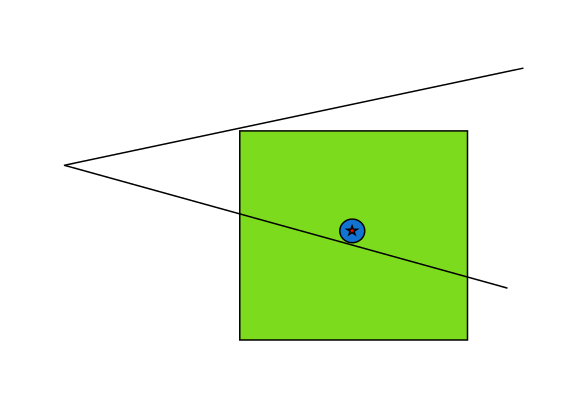
\includegraphics[width=200px]{images/small_circle.png}
    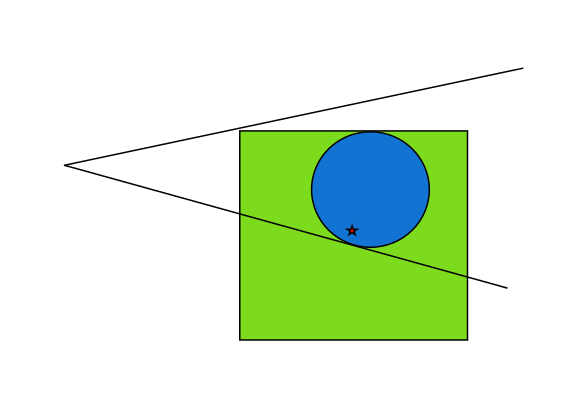
\includegraphics[width=200px]{images/shifted_center.png}
    \caption{When the current iterate is too close to a constraint, the circular trust region becomes too small. Shifting the trust region center helps remedy this. The star is the current iterate, the green is the outer trust region, and blue the inner.}
    \label{options_basis}
\end{figure}







\subsubsection{Ellipsoids}

In order to address this issue we considered using ellipsoidal trust regions.
Whereas the circle does not allow improvement when the current iterate lies along a constraint, an ellipsoid elongates along this constraint.
In figure \cref{ellipse_adv}, we have this type of iterate, but by using an ellipsoid we are still able to search towards the vertex of the feasible region.
\begin{figure}[h]
    \centering
    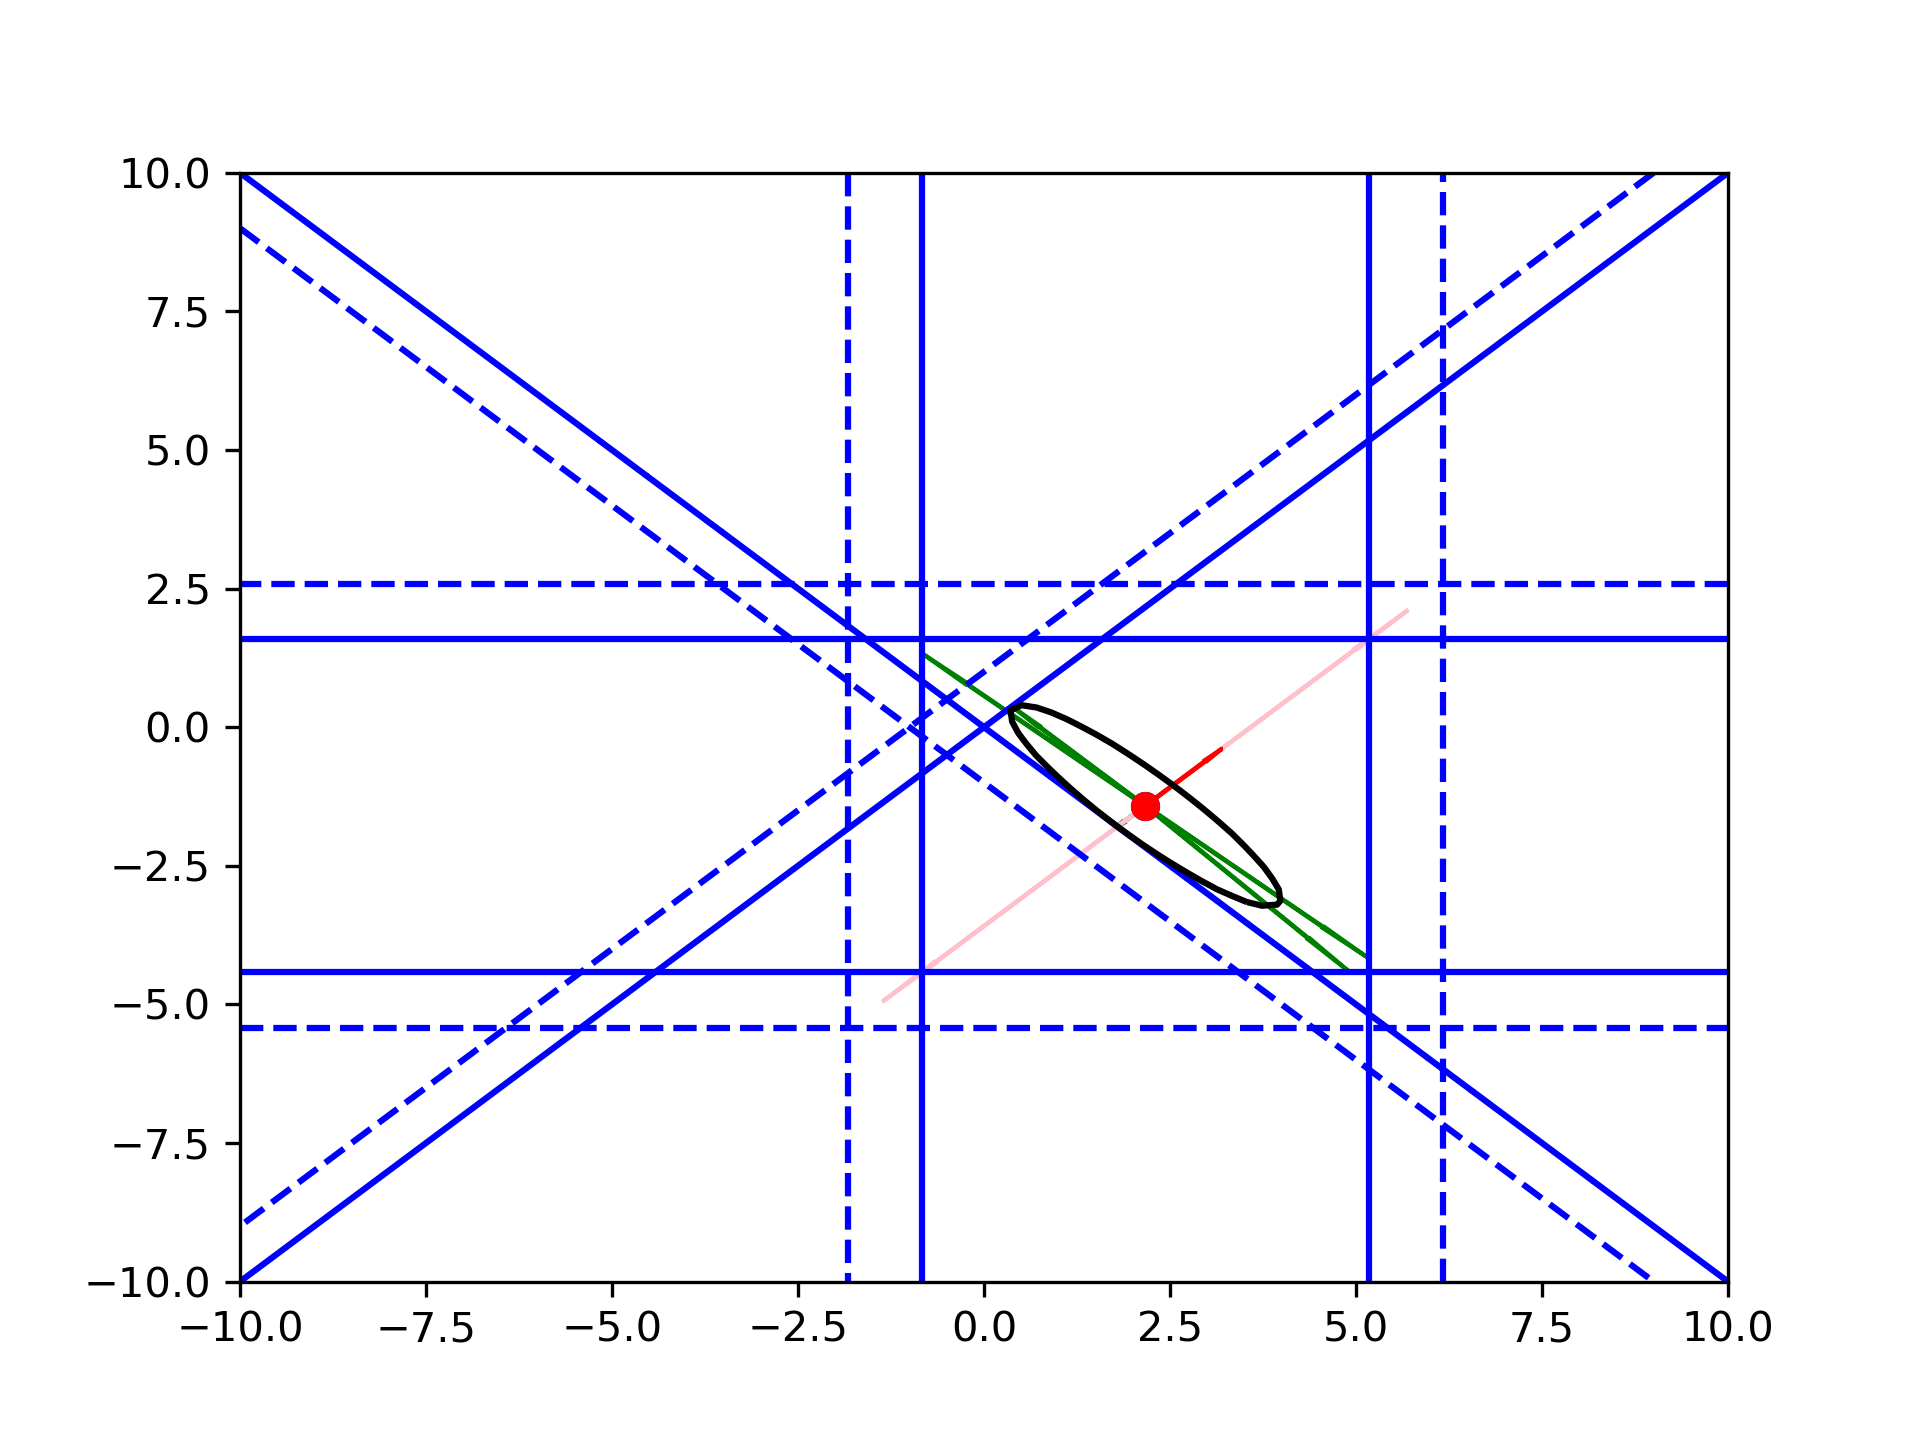
\includegraphics[scale=0.4]{images/advantage_of_ellipse_2.png}
    \caption{A nicer trust region}
    \label{ellipse_adv}
\end{figure}


More specifically, at iteration $k$, we choose a scaling factor $\pi^k$ and solve for an ellipsoid center $\mu^k$ and positive definite matrix $\qk$ to define an ellipsoid
$ \ellipsek = \{x \in \Rn \| \pi^k - \frac 1 2 (x - \mu^{k})^T\qk(x - \mu^{k}) \ge 0 \}$.
Of course, the simplest approach is to not change the center of the ellipsoid, but instead let $\mu^k = x^k$.



\subsubsection{Search Everything}

One approach is to search all possible centers within $ \feasible \cap \outertrk $.
That is, we solve:
$$\mu^k = \sup_{\mu \in \feasible \cap \outertrk} V(\mu)$$
where $V(\mu)$ is the volume of the ellipsoid defined in \cref{ellipse_1}.
%The search within the \emph{ConstructTrustRegion} is allowed to go anywhere within $ \feasible \cap \outertrk$.
This has the advantage that it captures much of the feasible region.
However, one problem with this search is that it can force the trust region away from the desired direction.
Notice that in \cref{ellipse_runs_away}, although the ellipsoid found has larger volume than before being shifted, this ellipsoid contains points farther from the corner containing the minimizer.

\begin{figure}[h]
    \centering
    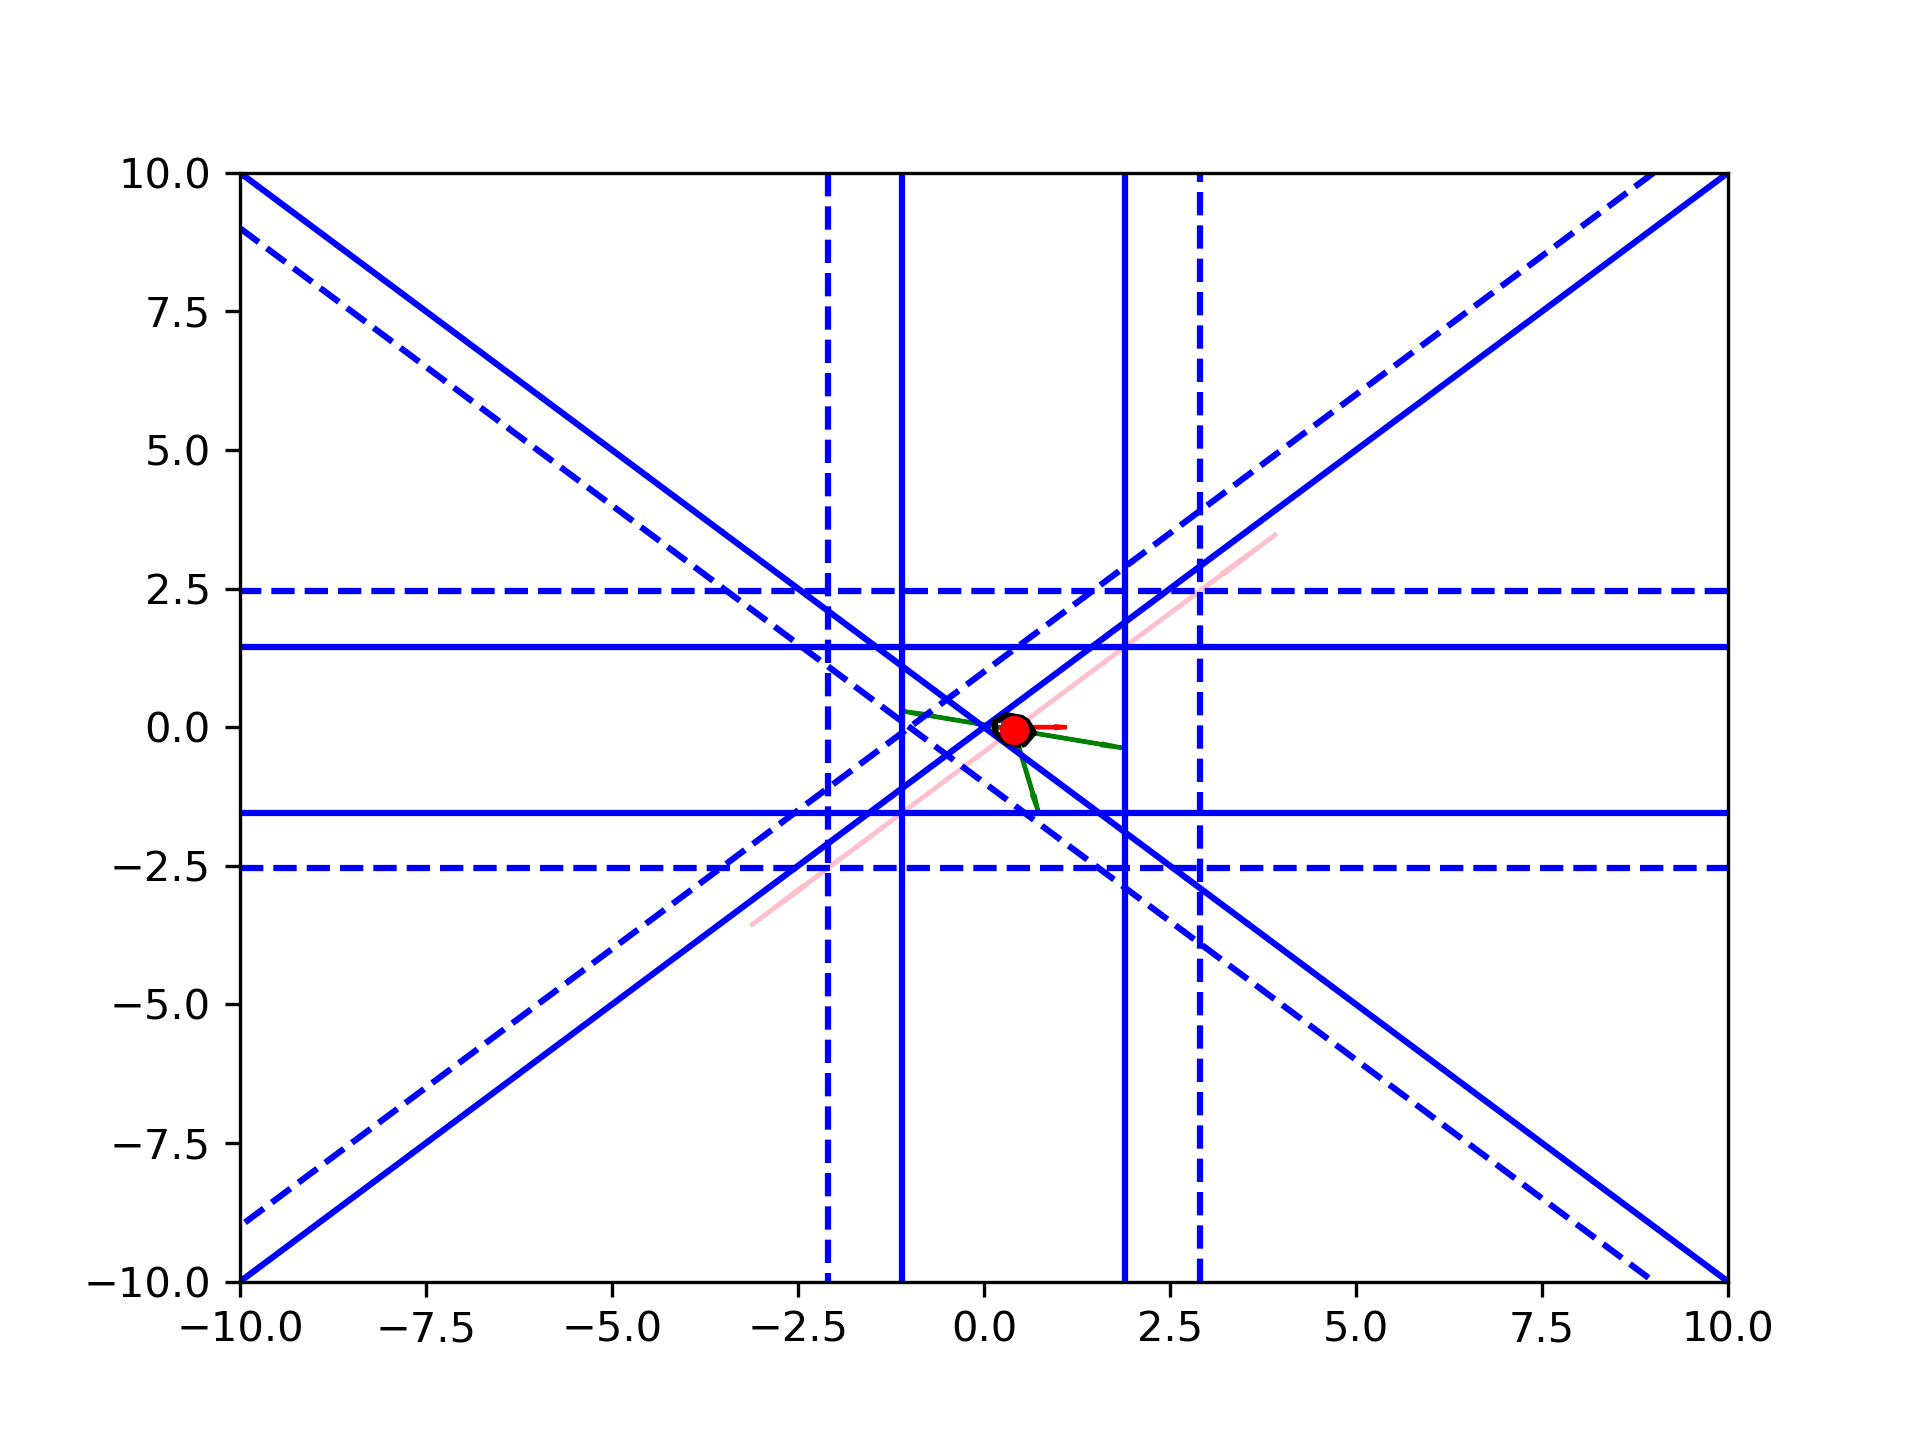
\includegraphics[scale=0.4]{images/everything_runs_1.png}
    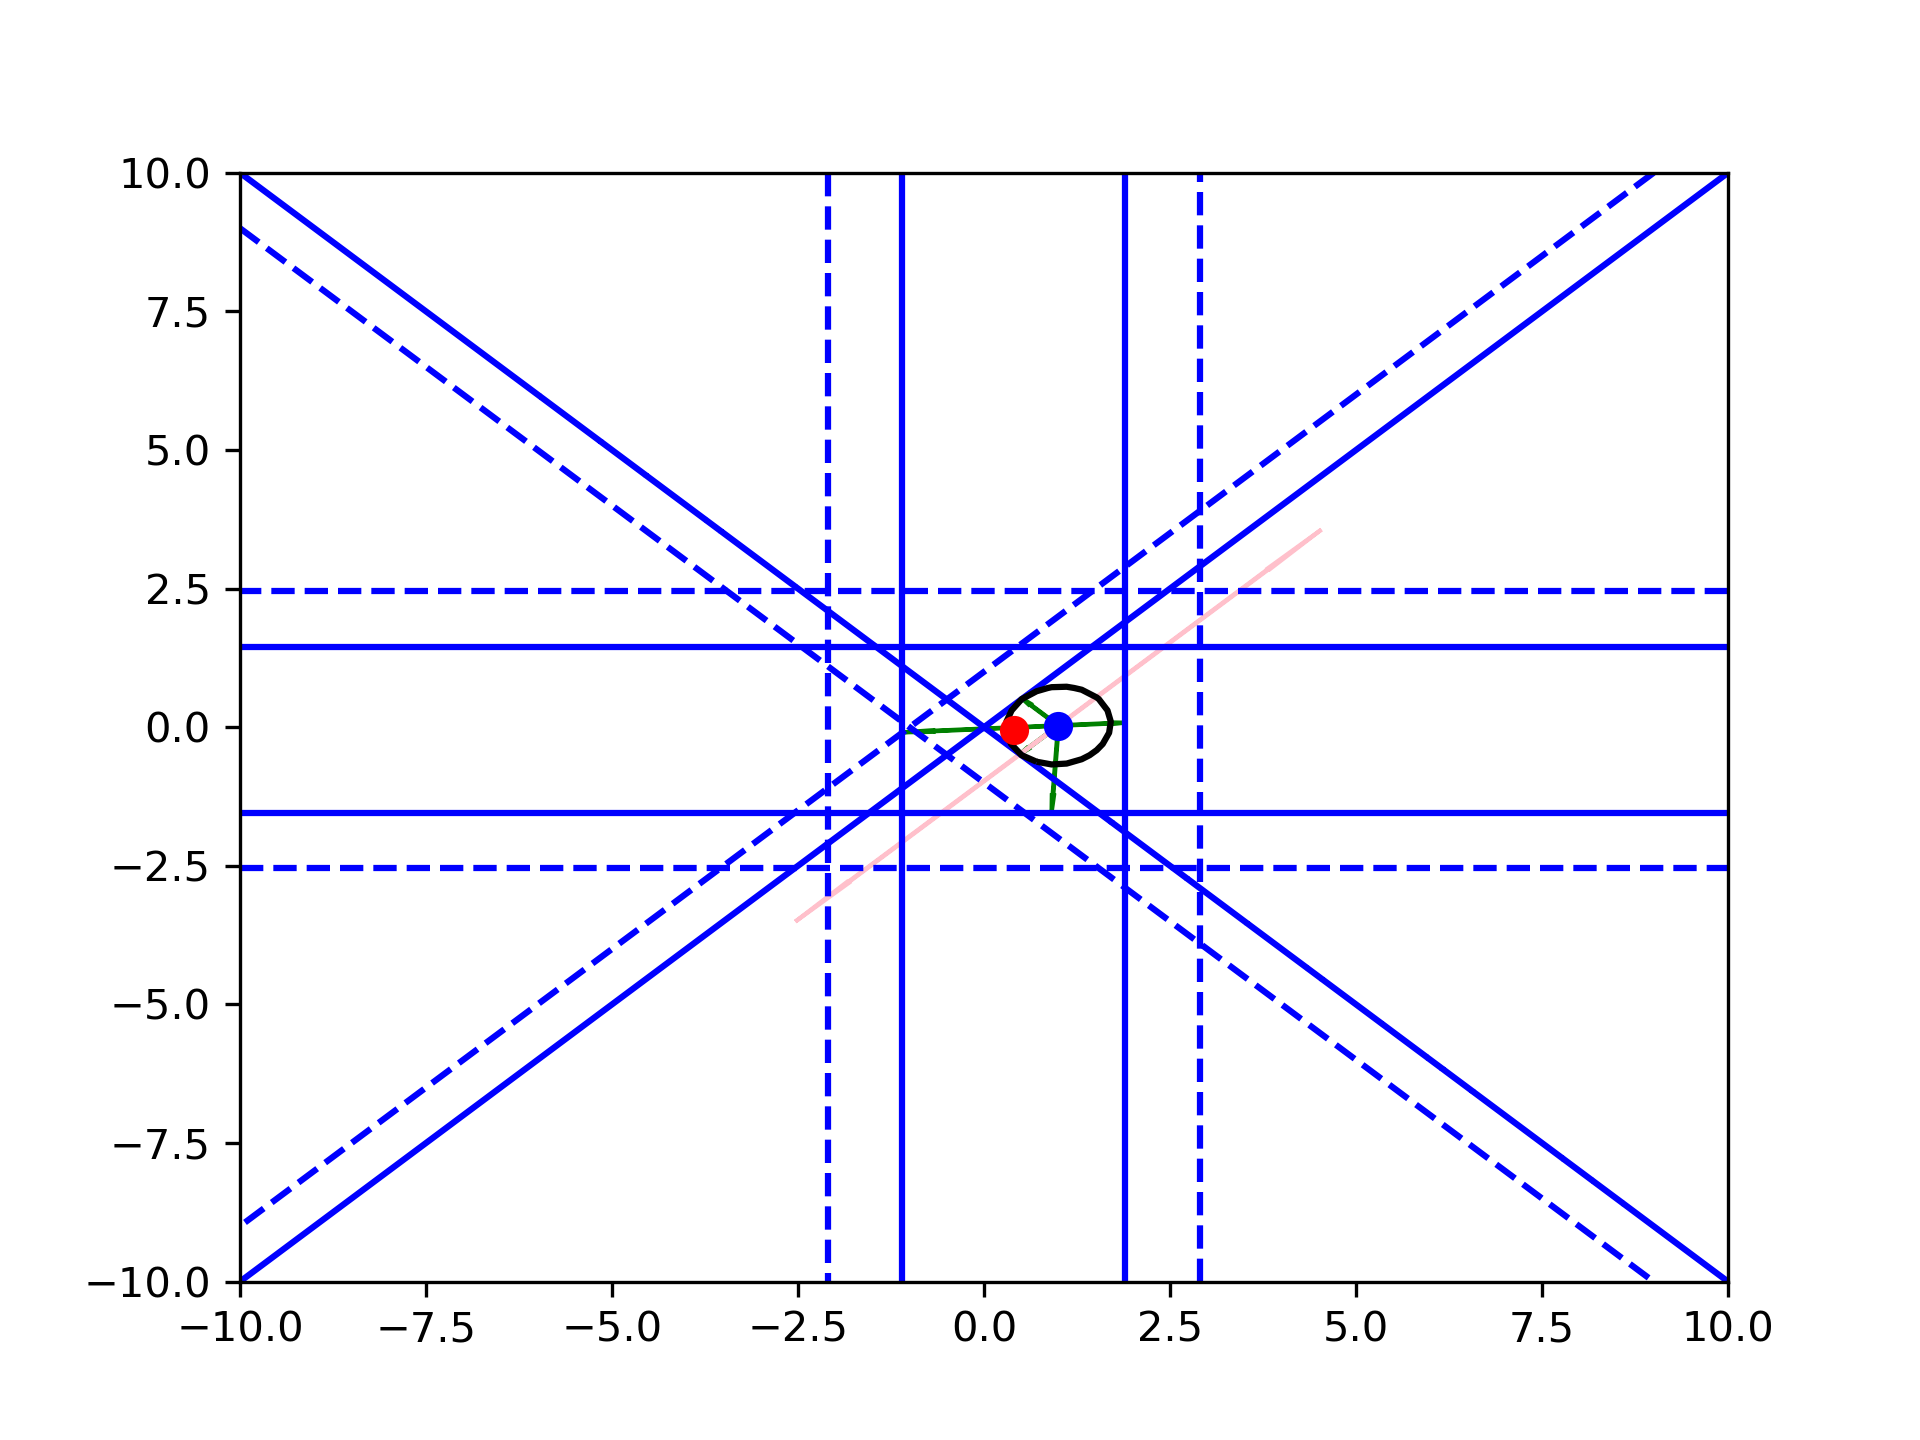
\includegraphics[scale=0.4]{images/everything_runs_2.png}
    \caption{Searching $\feasible$}
    \label{ellipse_runs_away}
\end{figure}


One attempt to fix this problem is by limiting the search direction for the center of the ellipsoid.


\subsubsection{Line Searches}
Although $\mfk$'s minimizer over $\outertrk$  can appear anywhere, there are some reasons for expecting it to be at a ``vertex."
If it lies in the interior, there is little need for using constrained approaches once near the solution.

%The ellipsoid with maximum volume, however, tends to lead $ \sampletrk $ away from vertices.
One way of trying to ensure a feasible direction towards a vertex, while still allowing a larger volume ellipsoid, is by limiting the search for the new center to lie on line segments starting at the current iterate $\xk$.

For example, our first attempt was to simply search a line directed orthogonally away from the closest constraint.
This has obvious problems as shown in \cref{first_line_search}, as we should avoid letting the new center get closer to another constraint:

\begin{figure}[h]
    \centering
    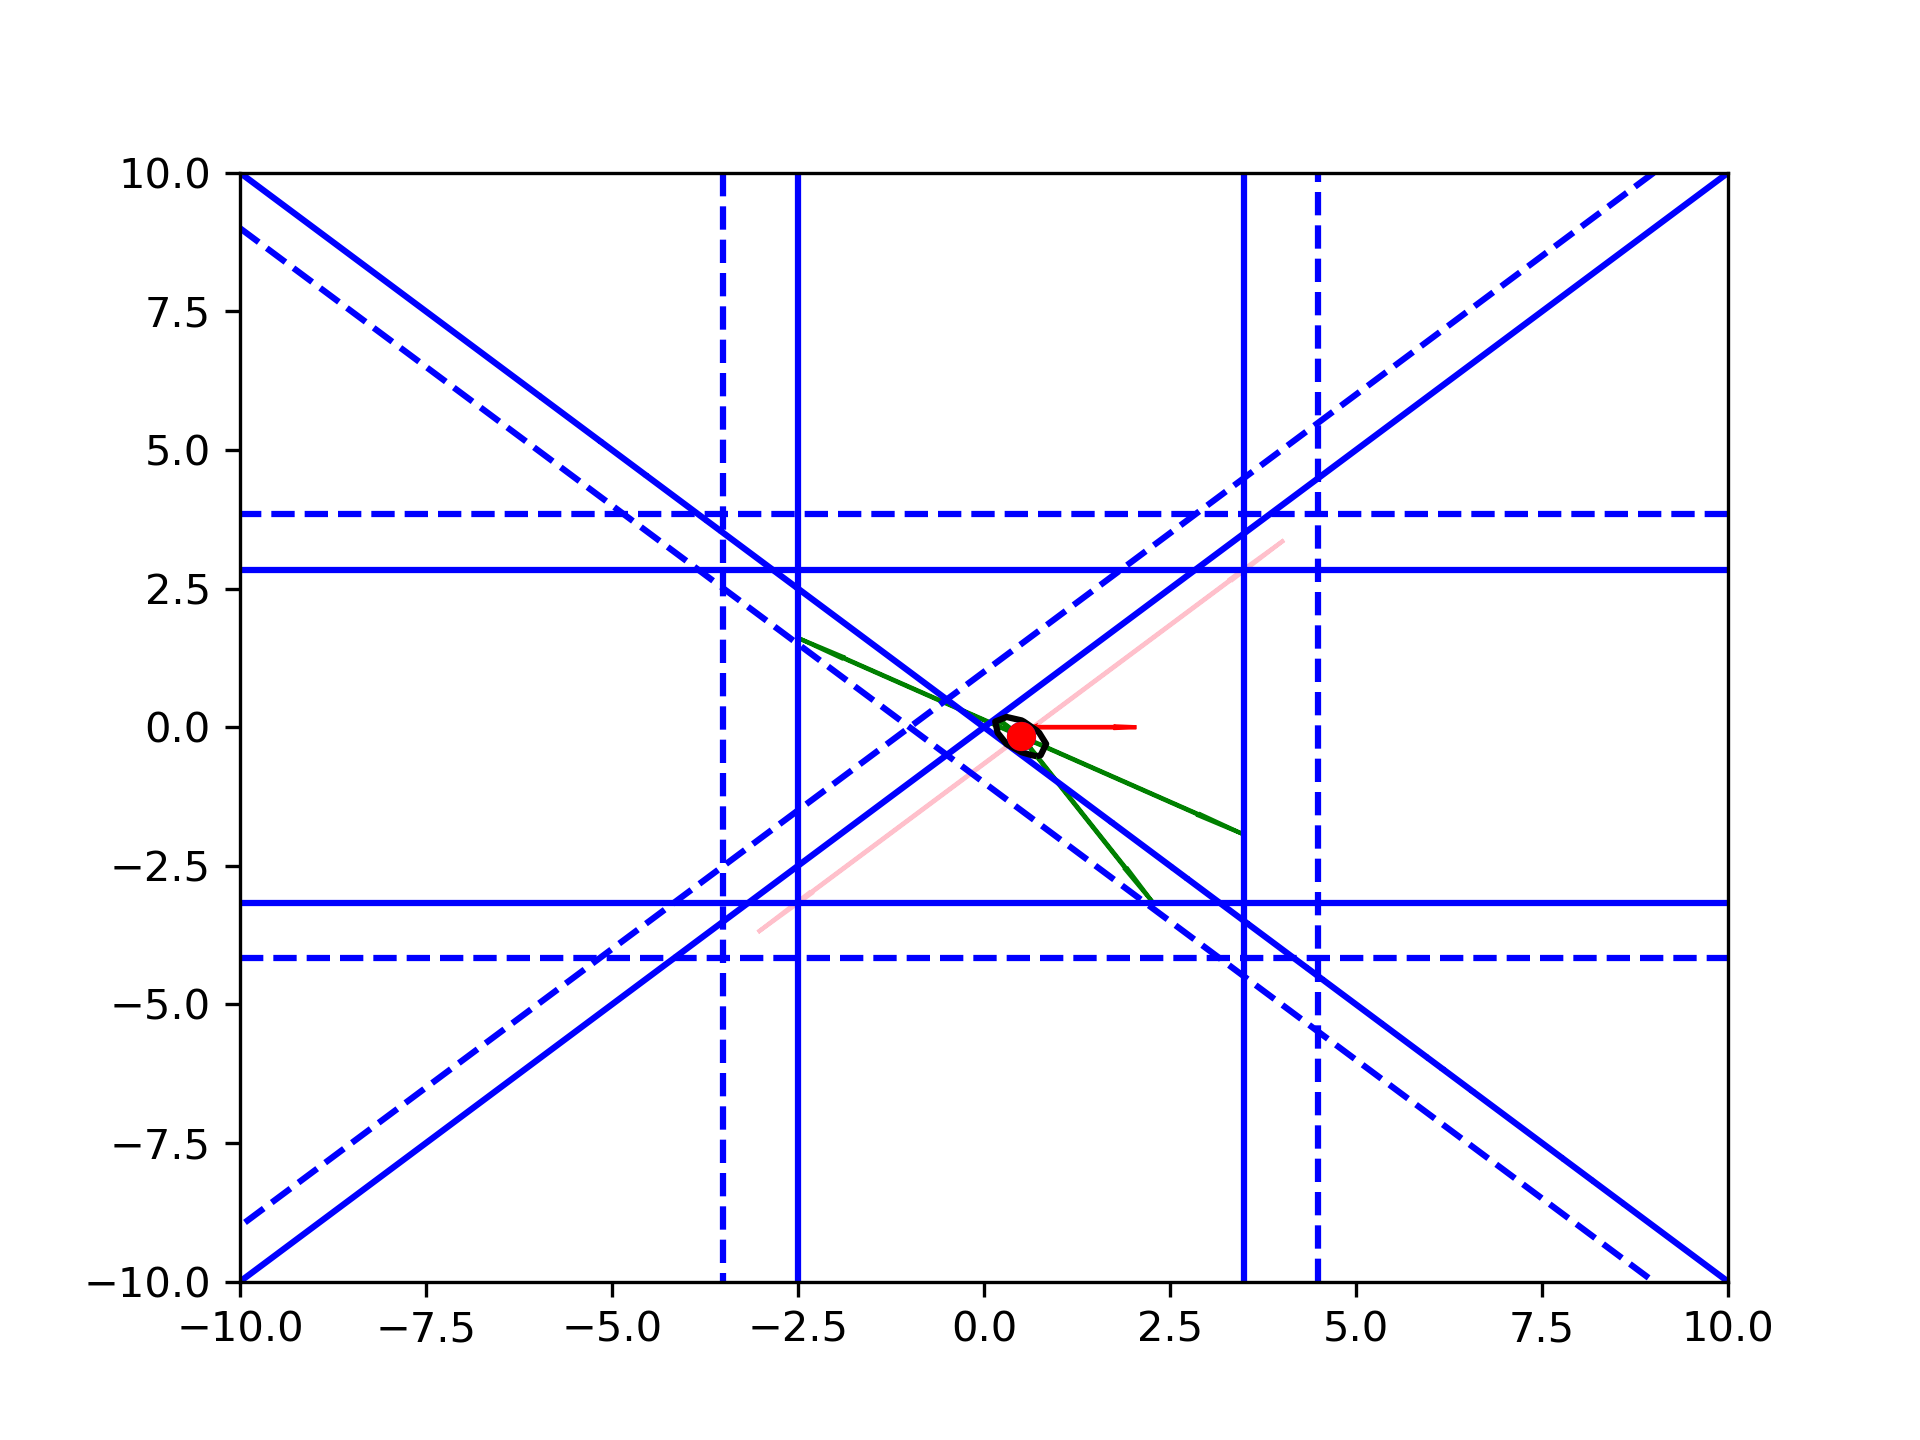
\includegraphics[scale=0.4]{images/line_1.png}
    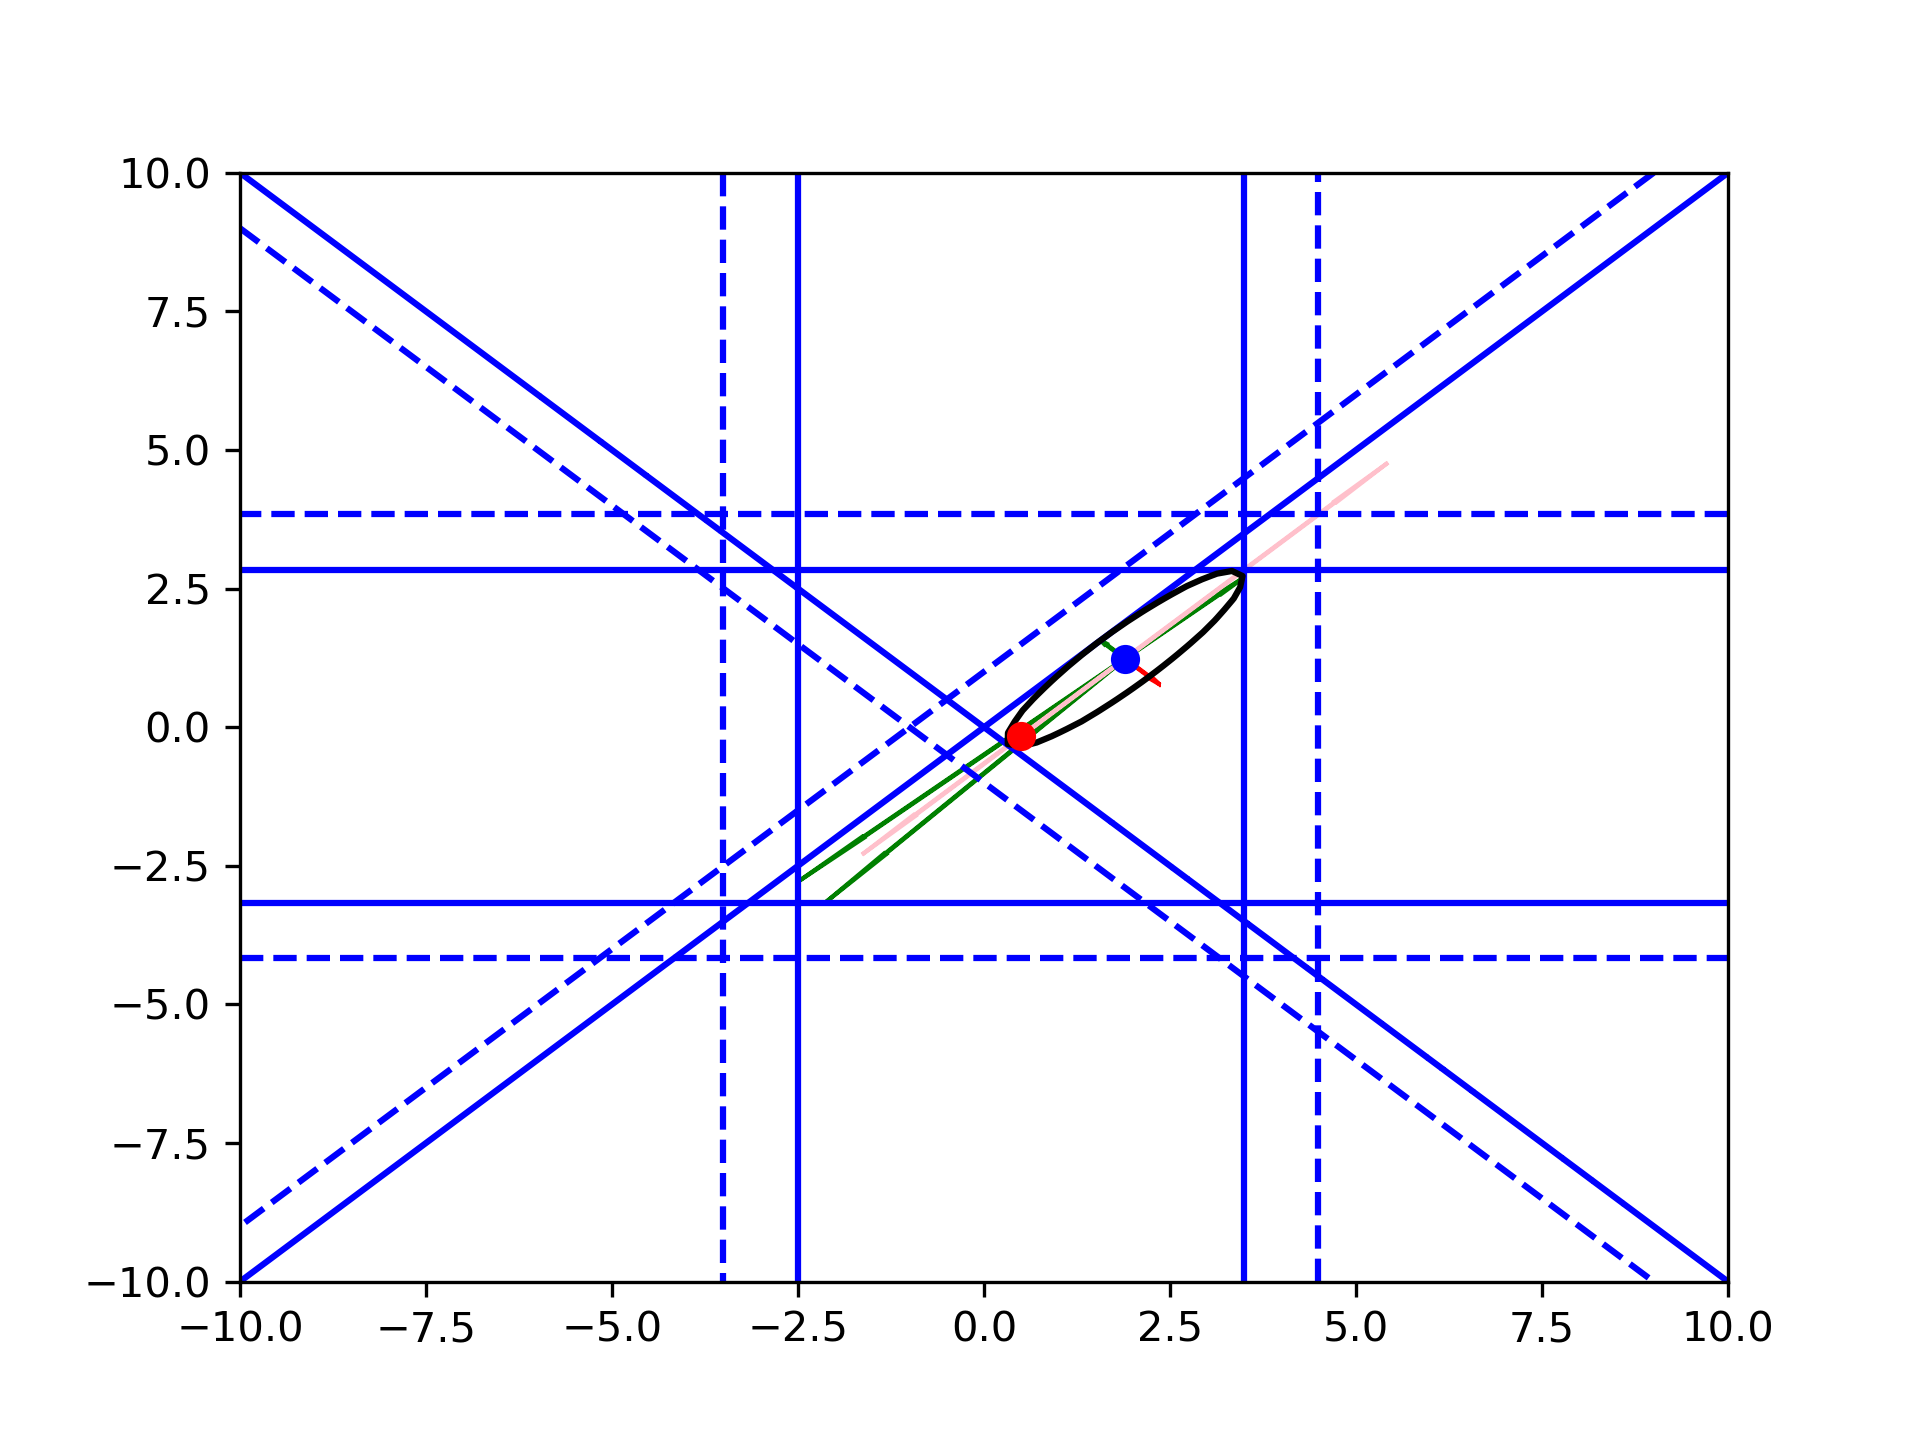
\includegraphics[scale=0.4]{images/line_2.png}
    \caption{Line searches}
    \label{first_line_search}
\end{figure}


For a given distance $d$, let the indices $i$ for which $\frac {|A_i x - b|}{\|A_i\|} \le d$


To fix this, we break the search space within the \emph{ConstructrustRegion} subroutine into segments based on the nearest constraints.
The algorithm works by choosing a set of up to $n_{\text{points}}$ points $s_1, s_2, \ldots, s_{n_{\text{points}}}$ that are each equidistant to a subset of the constraint's faces.
The center search then considers points along the line segments between these points.
% Namely, it starts at the current iterate and travels along a ray away from all the closest constraints until it reaches a point equidistant to yet another constraint.

More precisely, the first point is chosen to be the current iterate: $s_1 = \xk$.
The algorithm then repeats the following process for $i$ from $1$ to $n_{\text{points}}$.
First, compute the set of nearest constraints, where the distance from a point $x$ to a constraint $A_i$ is given by $d(A_i, x) = \frac {|A_i x - b|}{\|A_i\|}$.
While finding the next point $s_{i+1}$, let  $A_E$ be a normalized array of the equidistant faces $\{\frac{A_i}{\|A_i\|} | d(A_i, s_i) = \min_j d(A_j, s_i), i = 1, 2, \ldots, m\}$ and $b_E$ be the rows' corresponding values of $b$.
All other faces are called the remaining faces, and construct the matrix $A_R$ and vector $b_R$.
It then finds a search direction $p  = r{A_E}^T$ as a linear combination of the normal vectors to the equidistant faces.
%When the constraint violation of $s_i$ is non-zero, this search ray can be found by finding the point that doubles the current slack ${A_E}s_i-{b_E}$.
%This is given by $r{A_E}^T$ where $r$ solves the linear system ${A_E}(s_i + r{A_E}^T) - b_E = 2 ({A_E}n_i - b_E)$.
%If the current violation is zero, then the right hand side can be set to a vector of all ones to ensure that all slacks violations are the same: $A_E(s_i + r{A_E}^T) - b_E = 1$.
This search ray can be found by setting the slack to each equidistant face to a vector of all ones: $A_E(s_i + r{A_E}^T) - b_E = 1$.
We can travel along this ray until we reach a point that is the same distance to a remaining face.
Specifically, we can travel by 
\begin{align}
t = \argmin_j {\frac{d({A_E}_0, s_i) - d({A_R}_j, s_i)}{ {A_R}_j - d({A_E}_0) p} | ({A_R}_j - d({A_E}_0) p > 0 }. 
\end{align}

We can then set $s_{i+1} = s_{i} + t p$.

Of course, $n_{\text{points}}$ must be less than or equal to $n + 1$ in order for this to be defined.
Also, the algorithm must stop early if $A_E$ contains parallel faces.

% if we let $\nabla \modelconstrainti(\xk) = A_i$ be the $i$th row of $A$, then we define the distance from a search point $s$ so the $i$th constraint to be


This means that we can define a class of searches that each limit the number of line segments to search $n_{\text{points}}$.

In figure \cref{line_can_run}, the red line shows the line segments equidistant their closest constraints.
Notice that with two line segments, the algorithm can already choose new centers further from the vertex.

% TODO: REPLACE PICTURES
\begin{figure}[h]
    \centering
    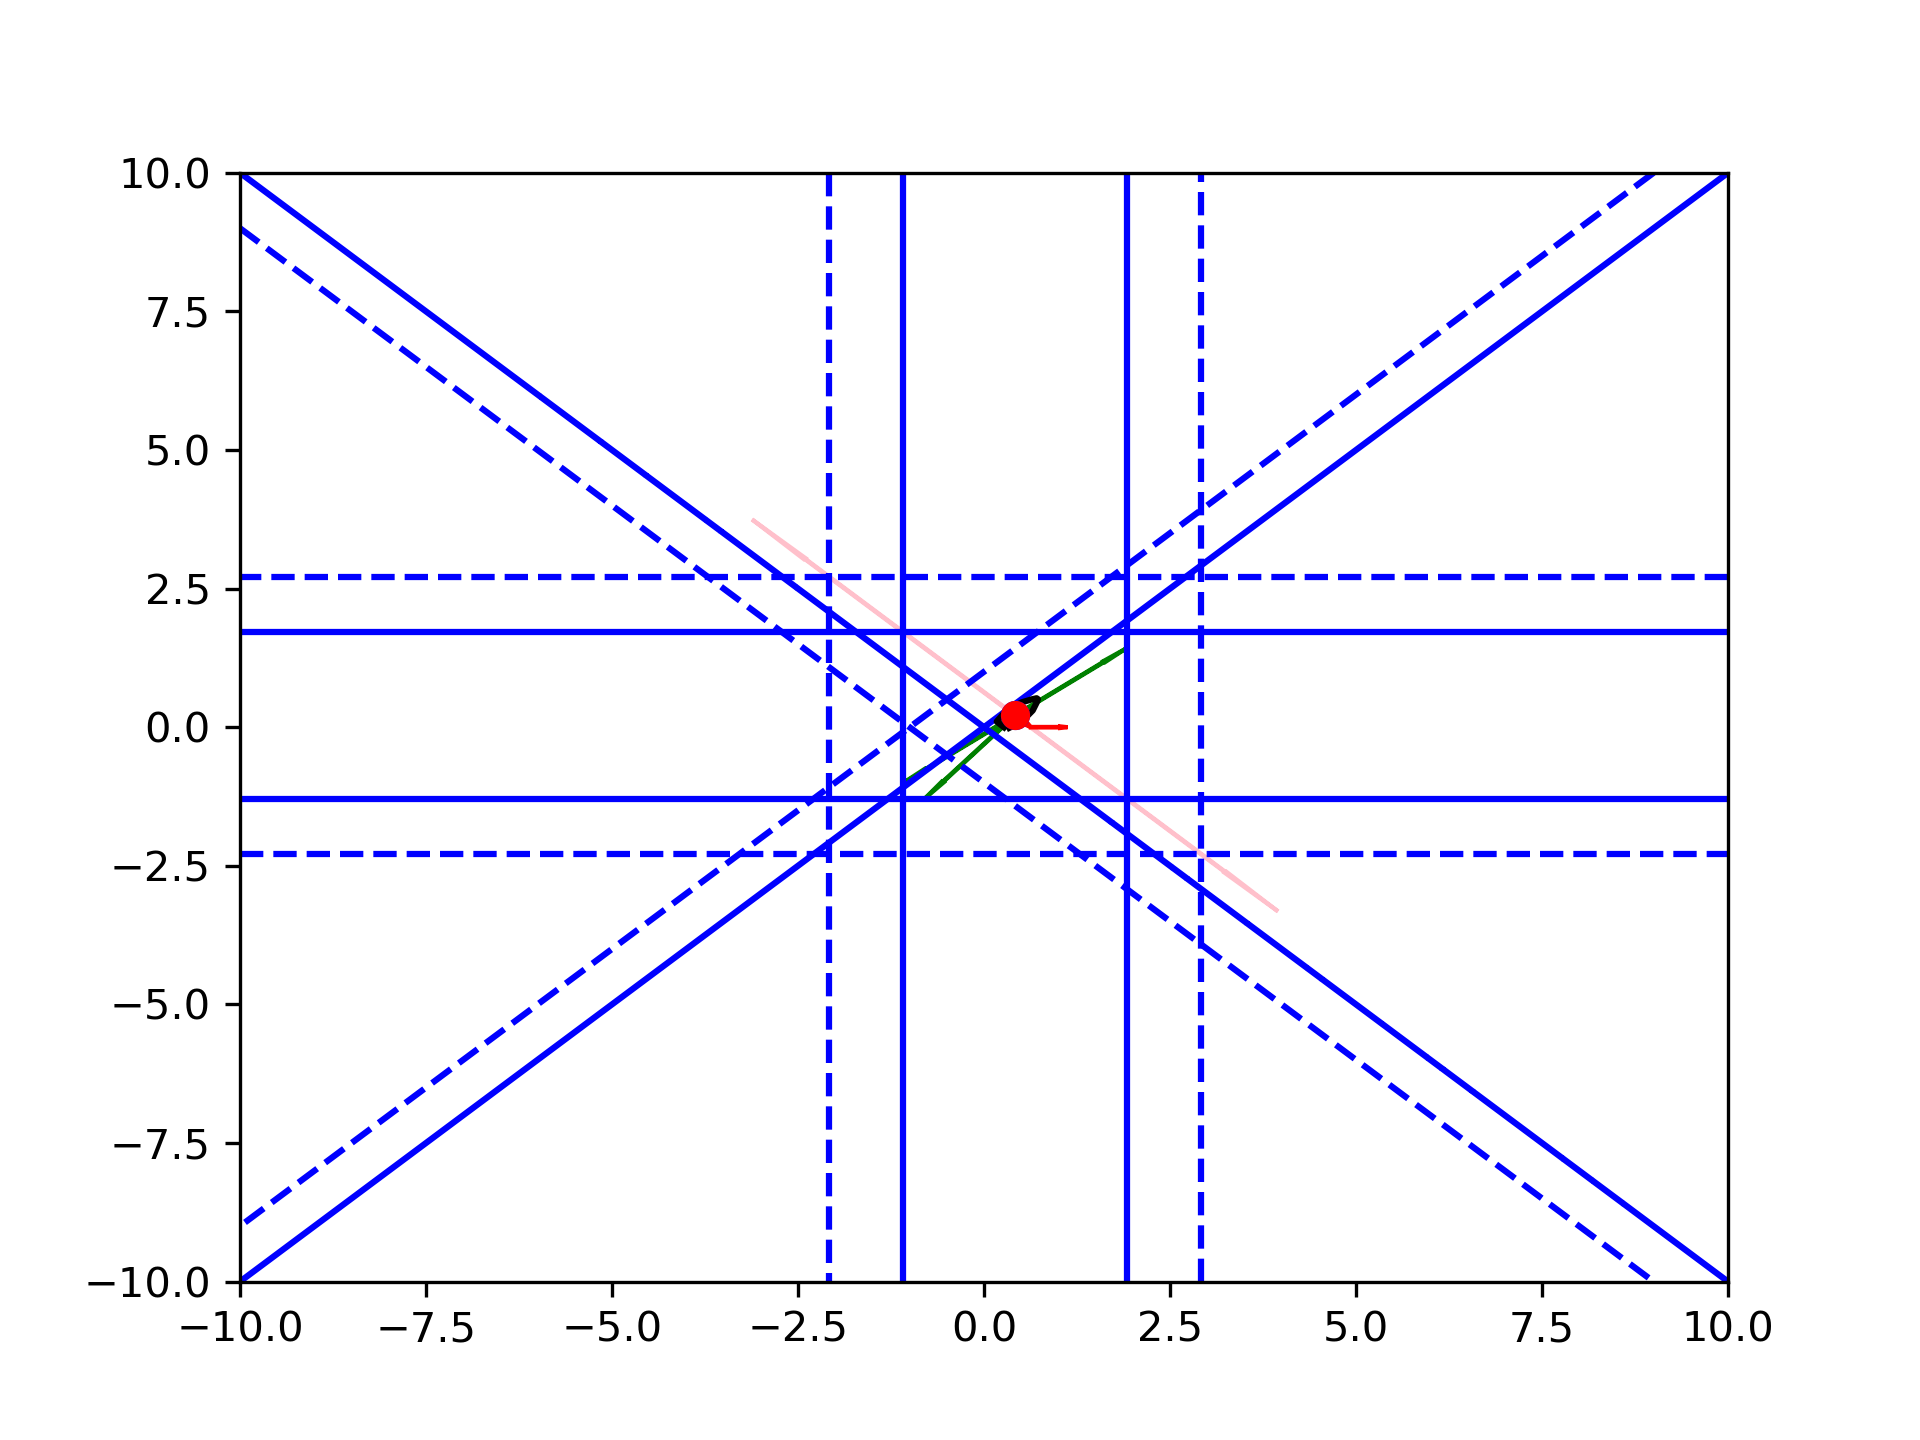
\includegraphics[scale=0.4]{images/run_away_1.png}
    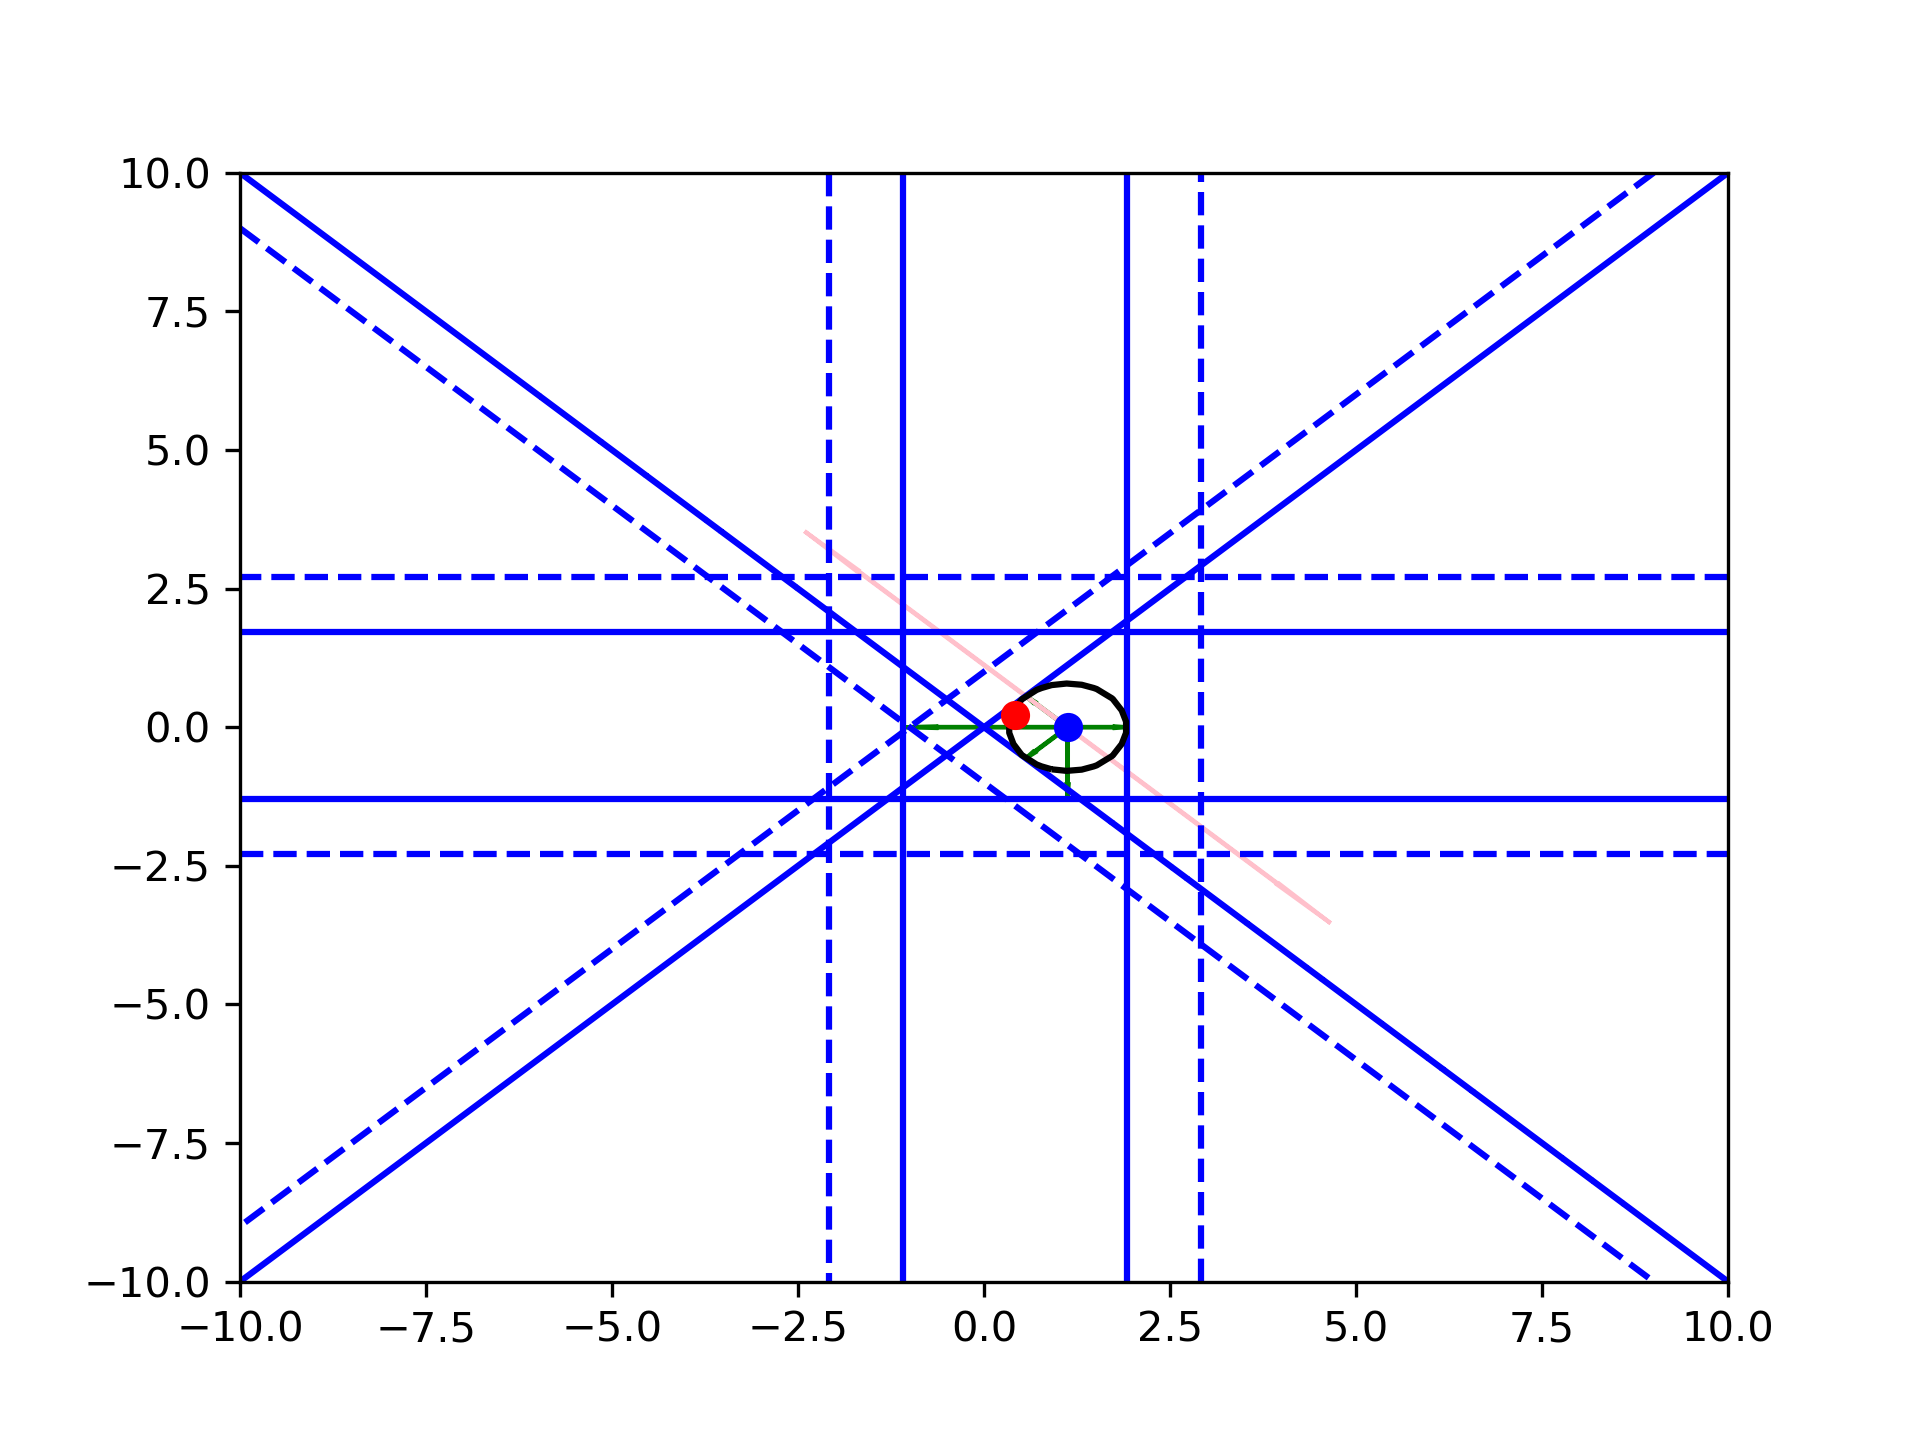
\includegraphics[scale=0.4]{images/run_away_2.png}
    \caption{Ellipse runs away from the optimizer}
    \label{line_can_run}
\end{figure}







=========

This section describes strategies for choosing the center $\mu^k$ for the ellipsoid $E^k$.  At issue is the fact that if the center of the ellipsoid is too close to the boundary of the feasible region, then the condition number of $Q^{k}$ may be unacceptably large.  We there   There are several issues at play:
\begin{itemize}
    \item The ellipsoid should include the current iterate (or maybe not).
    \item We want the ellipsoid
\end{itemize}


\subsubsection{Ellipsoid Choices}

There are a number of issues to be solved to define this ellipsoid:
\begin{itemize}
\item How do we ensure that $\xk \in \ellipsek $?
\item How do we choose $\ellipsek$ in such a way that it does not limit travel along a decent direction?
\item How do we choose the center of the ellipsoid $\mu^k$?
\end{itemize}

% \item How do we choose $\ellipsek$ to make the  ellipsoid as large as possible while ensuring that $ \ellipsek \subset \outertrk \cap \feasible $?

If $\xk \not \in \searchtrk $, the ellipse may not even contain a point with any reduction.
Thus, we have implemented a few ways of ensuring the current iterate is within the search trust region.
This can be done by either of the following two options:
\begin{itemize}
\item Adding a constraint to the ellipsoid problem to include the original point.
\item Expand the size of the ellipsoid.
\end{itemize}

%IMAGES GO HERE

\paragraph{Adding a constraint.}
In order to include the original point as a constraint, we add a constraint to the definition of the ellipsoid of the following form:
$$ \pi^k - \frac 1 2 (x^k - \mu^{k})^T\qk(x^k - \mu^{k}) \ge 0. $$
Constraints of this nature make finding the ellipsoid much more expensive.
This is because the optimization problem we construct uses ${\qk}^{-1}$ as decision variables, so that constraints in terms of $\qk$ must model matrix inversion.

\paragraph{Increase the size.}
An alternative is to scale $\qk$ by a constant.
We use the scaling factor $\pi^k$ defined by

$$\pi^{(k)} = \max \{1, \frac 1 {2} (x^{k} - \mu^{k})^T \qk (x^{k} - \mu^{k})^T \}$$

and let the ellipsoid be:
$$\ellipsek = \{x \in \Rn | 1 - \frac 1 {2\pi^k} (x - \mu^{k})^T \qk (x - \mu^{k}) \ge 0\} $$
However, this means that in general $\ellipsek \not \subset \feasible$ so that the trust region subproblem must contain constraints for both the ellipsoid and the feasible region: $\searchtrk = \ellipsek \cap \domain$.

To help mitigate the second issue, we maximize the volume of the ellipsoid.
However, the choice of ellipsoid center can still limit travel along a decent direction.
Choosing the best center is the topic of the next section.\





\subsection{Algorithm Components}

Before describing the algorithm, we discuss several components referenced within an algorithm template.

\subsubsection{Criticality Measure}

In order to define stopping criteria for the algorithm, we introduce a criticality measure $\chi$ which goes to zero as the iterates approach a first order critical point.
When the criticality measure is small, we must also decrease the trust region radius.
Once this has reached a small enough threshold $\tau_{\chi}$ and the trust region is small enough ($\Delta_k < \tau_{\Delta}$), we can terminate the algorithm.
For now, our algorithm is designed to work with convex constraints, so we employ a classic criticality measure discussed in \cite{ConnGoulToin00} of
\begin{align}
\label{critical}
\chik = \|\xk - \text{Proj}_{\feasible}(\xk- \nabla \mfk(\xk))\|
\end{align}
The first order optimality conditions for $x^{\star} \in \Rn$ to by a local optimum of $f$ is that $x^{\star}$ satisfies
\begin{align*}
x^{\star} = \text{Proj}_{\feasible}\left(x^{\star} - \nabla f(x^{\star})\right).
\end{align*}
For linear constraints, this condition is necessary and sufficient.
Thus, our criticality measure measures how far the current iterate is from satisfying the first order optimality conditions for $\xk$ to be a optimum of $\mfk$.
In turn, as $\dk \to 0$, the model $\mfk$ better approximates $f$ and $\xk$ approaches an optimum of $f$.

\subsubsection{Assessing Model Accuracy and Radius Management}

Each iteration that evaluates a trial point must also test the accuracy of the model functions.
To test the accuracy, we calculate a quantity
\begin{equation}
\label{rho}
\rho_k = \frac{f(\xk) - f(\xk+\trialk)}{\mfk(\xk) - \mfk(\xk+\trialk)}
\end{equation}
which measures the actual improvement over the predicted improvement.
A small $\rho_k$ implies the model functions are not sufficiently accurate.
Values of $\rho_k$ close to $1$ imply that the model accurately predicted the new objective value.
A large $\rho_k$ implies progress minimizing the objective although the model was not accurate.
This has been widely used within trust region frameworks such as \cite{Conn:2000:TM:357813} and within a derivative free context \cite{DUMMY:intro_book}.
The user supplies fixed constants $0 < \gammasm \le \gammabi \le 1$ as thresholds on $\rho_k$ and $0 < \omega_{\text{dec}} < 1 \le \omega_{\text{inc}}$ as decrement or increment factors to determine the trust region update policy.


\subsection{Trust Regions}
Our algorithm maintains up to three trust regions.
The outer trust region is an $L_1$ ball of radius $ \dk $ defined by
\begin{equation}
\label{trust_region_outer}
\outertrk = B_{\infty}(\xk,\dk) = \{x\in \Rn | \; \xki - \dk \le x_i \le \xki + \dk \quad \forall 1\le i \le n\}.
\end{equation}

Note that the outer trust region may include infeasible points.
To ensure feasibility of all sample points, we construct an inner trust region for sample points $ \sampletrk $  satisfying 
$\sampletrk \subset \outertrk \cap \feasible$ and $\xk \in \sampletrk $.
However, we do not want to limit the search for a new iterate to the same trust region we use to construct the model.
This means we introduce another trust region $ \searchtrk $ that also satisfies $ \searchtrk \subset \outertrk \cap \feasible$ and $\xk \in \searchtrk $ for the trust region subproblem.

\paragraph{The Sample Region}
\label{sample_region_choices}
We consider general strategies for constructing $ \sampletrk $ and $ \searchtrk $.
\begin{itemize}
\item[1.] Take 
\begin{align}
\label{redpill} \sampletrk = \searchtrk = \outertrk \cap \feasible.
\end{align} This results in a polyhedral trust region, so we refer to this approach as the \emph{Polyhedral Trust Region Approach}.
% \item[2.] Let $\label{hybrid} \sampletrk \subseteq \searchtrk = \outertrk \cap \feasible $ where $\sampletrk$ has an ellipsoidal shape. This is referred to as the \emph{Hyrbid Trust Region Approach}
\item[2.] Force 
\begin{align}\label{bluepill} \sampletrk \subseteq \searchtrk \subseteq \outertrk \cap \feasible
\end{align} where $\sampletrk$ has an ellipsoidal shape. This is referred to as the \emph{Ellipsoidal Trust Region Approach}
\end{itemize}

The advantage of the ellipsoidal trust region approach \cref{bluepill} is that we can reuse classical methods for ensuring good geometry.
We can construct $\sampletrk$ to be ellipsoidal and use efficient algorithms within \cite{DUMMY:intro_book} to satisfy \cref{accuracy}.
However, we must be careful while choosing $ \searchtrk$ to allow sufficient reduction when we solve the trust region subproblem using the inner trust region.
The search trust region is used while selecting the next iterate:
\begin{align*}
\trialk = \argmin_{\trialk \in \searchtrk} \mfk(\xk + \trialk).
\end{align*}

\paragraph{The Search Region}
\label{search_region_choices}
When using the ellipsoidal trust region approach, we have two choices for this trust region.
We can take
\begin{align}
\searchtrk = \sampletrk \label{search_a_little}
\end{align}
or
\begin{align}
\searchtrk = \outertrk \cap \feasible \label{search_a_lot}.
\end{align}
Namely, in \cref{search_a_little} with an ellipsoidal inner trust region, we still have an option to select our trial point from the entire $\trialk \in \outertrk \cap \feasible$.

To complete the polyhedral trust region approach \cref{redpill},
we need some redefinition of poisedness for polyhedral shapes.
However, since the trust region is larger, it is easier to ensure sufficient reduction.
This strategy has the drawback that it will yield sample points close to the boundary of the feasible region.
This may cause more infeasible evaluation attempts when we use models to approximate black-box constraints this may.

The classical methods for ensuring good geometry require an optimization call to the model functions over a sphere.
This is no longer possible in the polyhedral trust region approach.
However, the bounds produced over the entire trust region may also be stronger than required as the models will only be used on the feasible region.
This may mean the geometric requirements can be reduced.

Within our algorithm, if $ \outertrk \subseteq \feasible$ we can set $ \sampletrk $ to be a sphere.
This saves the computation of $ \sampletrk $ when it is not needed, as there are no nearby constraints.









\section{Algorithms}

\subsubsection{Sufficient Model Reduction}

To ensure sufficient reduction of the objective's model function during each iteration, we impose the following efficiency condition:
\begin{equation}
\label{efficiency}
\mfk(\xk) - \mfk(\xk + \trialk) \ge \kappa_f \chi_k \min\left\{ \frac{\chi_k}{1+\|\nabla^2 \mfk(\xk)\|}, \dk, 1 \right\}
\end{equation}
where $\kappa_f$ is a constant independent of $k$.
This is widely used within trust region frameworks such as \cite{conejo.karas.ea:global} and \cite{Conn:2000:TM:357813}.
It can be shown that the \emph{generalized Cauchy point} satisfies this condition \cite{Conn:2000:TM:357813}.



\subsection{Algorithm Template}

We follow an algorithm template described in \cite{doi:10.1080/10556788.2015.1026968}, where variations of the algorithm have different choices of $ \sampletrk $ implemented in a \emph{ConstructTrustRegion} subroutine.
The different versions are described in the remainder of this section.

% HOW ABOUT JUST MAKE $\eta > 0$?


\begin{algorithm}[H]
    \caption{Always-feasible Constrained Derivative Free Algorithm}
    \label{constrained_dfo}
    \begin{itemize}
        \item[\textbf{Step 0}] \textbf{(Initialization)} \\
            Initialize tolerance constants 
            $\tolcrit \ge 0$,
            $\tolrad \ge 0$,
            starting point $x^{(0)} \in \feasible$,
            initial radius $\Delta_0 > 0$,
            iteration counter $k=0$,
            $0 < \omegadec < 1 \le \omegainc$,
            $0 < \gammasm < \gammabi \le 1$,
            $\alpha > 0$,
            $k \gets 1$,
            $0 < \omegadec < 1 \le \omegainc$,
            $0 < \gammasm < \gammabi < 1$.
            
        \item[\textbf{Step 1}] \textbf{(Construct the model)} \\
            $ \sampletrk \gets $ \Call{ConstructTrustRegion}{$\dk, \xk$}.
            Ensure that the sample points are poised with respect to $ \sampletrk $ for \cref{accuracy} by calling \cref{model_improving_algorithm}.
            Construct $\mfk$ as described in \cref{reg} to construct $\mfk(x)$.
        
        \item[\textbf{Step 2}] \textbf{(Check stopping criteria)} \\
            Compute $\chi_k$ as in \cref{critical}. \begin{itemize}
                \item[] If $ \chik < \tau_{\xi} $ and $\dk <\tau_{\Delta}$ then return $\xk$ as the solution.
                \item[] Otherwise, if $\dk > \alpha \chik$ then 
                $\Delta_{k+1} \gets \omegadec\dk$, 
                $x^{(k+1)} \gets \xk$,
                $k \gets k+1$ and go to Step 1.
            \end{itemize}
        
        \item[\textbf{Step 3}] \textbf{(Solve the trust region subproblem)} \\
            Compute $\trialk = \min_{s \in \searchtrk} \mfk(\xk + \trialk)$.
            % \item[] This can also be $\trialk = \min_{s \in \outertrk \cap \feasible} \mfk(\xk + \trialk)$ depending on the choice made in \cref{which_trust_region}.
            
        \item[\textbf{Step 4}] \textbf{(Test for improvement)} \\
            Evaluate $f(\xk + \trialk)$ and evaluate $\rho_k$ as in \cref{rho} \begin{itemize}
                \item[] If $\rho_k < \gammasm$ then $\xkpo=\xk$ (reject) and $\Delta_{k+1} = \omegadec\dk$
                \item[] If $\rho_k \ge \gammasm$ and $\rho < \gammabi$ then $\xkpo=\xk+\trialk$ (accept), $\Delta_{k+1} = \omegadec\dk$
                \item[] If $\rho_k > \gammabi$ then $\xkpo=\xk+\trialk$ (accept), $\Delta_{k+1} = \omegainc\dk$
                % and either increase the radius or decrease if $\nabla \mfk(\xk)$ is small
            \end{itemize}
            $k \gets k+1$ and go to Step 1.
    \end{itemize}
\end{algorithm}
 

Much of the work is deferred to the \emph{ConstructTrustRegion} subroutine.
We will describe several different approaches for this subroutine.

\subsection{Polyhedral Trust Region Approach}
One simple approach to handle partially-quantifiable constraints is to maintain the same trust region as the classical algorithm, but avoid letting points fall outside the feasible region within the model improvement algorithm \cref{model_improving_algorithm}.
That is, we add the constraints $\mcik(x) \le 0 \forall i \in \mathcal{I}$ and $\mcik(x) = 0 \forall i \in \mathcal{E}$ to the model improvement algorithm while selecting new points.
This constrains the new points to also lie within the current model of the trust region in \cref{model_improving_algorithm}, Step 2.
The search space for this optimization problem will be the feasible region intersect the trust region: $\feasible \cap \outertrk $.

The challenge lies in finding sufficiently poised sample points.
Note that \cref{model_improving_algorithm} uses a parameter $  \ximin $ as a lower bound of the pivot values of the Vandermonde matrix.
For unconstrained problems, this approach could always find a pivot value for any $ \ximin \in (0,1)$ because it optimized over a sphere.
However, when requiring points to live within $ \feasible \cap \outertrk $, it can happen that even after replacing a point, we still have not satisfied this bound.
In \cref{lspc}, for some values of $  \ximin $, there is no point in $ \feasible \cap \outertrk $ that will leave a sufficiently large pivot.

\begin{figure}[h]
    \centering
    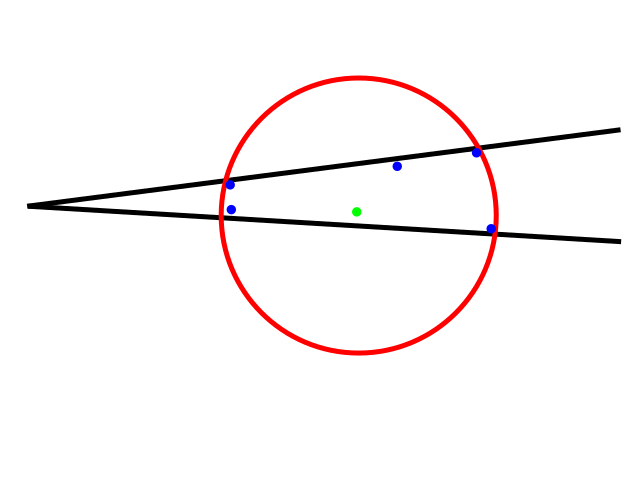
\includegraphics[scale=0.4]{images/bad_lambda.png}
    \caption{Limited sample point choice}
    \label{lspc}
\end{figure}

%As the number of dimensions grows the ratio of volume of the trust region intersect the feasible region to the feasible region can become smaller.

One way to handle this is to introduce a $\xi_{\text{cur}}$ which is allowed to decrease.
(Possibly, until a threshold is reached for maintaining a fixed $\Lambda$.)
If the new point does not improve the geometry of the set significantly, then there is no other point that would do better.
To test this, we introduce a constant $\delta_{\text{improv}}>0$ and require a new point to increase the current pivot by a factor greater than $\delta_{\text{improv}}$.
If the new point does not satisfy this test, we proceed with our current point and possibly decrease $\xi_{\text{cur}}$.
The new modified improvement algorithm is described in \cref{modified_model_improving_algorithm}:

\begin{algorithm}[H]
    \caption{Modified Model Improvement Algorithm}
    \label{modified_model_improving_algorithm}
    \begin{itemize}
        \item[\textbf{Step 0}] \textbf{(Initialization)} \\
            Initialize $i=1$.
            If the current sample set does not have $p$ points, repeat one of the current points. 
            Construct the Vandermonde matrix $V_{i,j} = \phi_j(\frac 1 {\Delta}(y^i - y^0))$.
            Initialize $0 < \ximin < \xi_{\text{desired}}$, $0 <\delta_{\text{improv}} < 1$,
            $  \xi_{\text{cur}} = \xi_{\text{desired}}$.
            
        \item[\textbf{Step 1}] \textbf{(Pivot)} \\
            Swap row $i$ with row $i_{\max} = \arg \max_{j|j\ge i} V_{j,i} $
        
        \item[\textbf{Step 2}] \textbf{(Check threshold)} \begin{itemize}
                \item[] If $|V_{i,i}| \ge \xi_{\text{cur}} $ then go to Step 3
                \item[] $ \hat y = \arg\max_{t \in \sampletrk \cap X} |\phi_i(t)|$
                \item[] If $\label{impossibly_poised} |\phi_i(\hat y)| < \ximin$ then \textbf{Stop}: the algorithm failed
                \item[] If $\xi_{\text{cur}} - |\phi_i(\hat y)| > \delta_{\text{improv}} \xi_{\text{cur}}$ then replace $V_{i,j}$ with $\phi_j(\hat y)$ and $\xi_{\text{cur}} \gets |\phi_i(\hat y)|$
            \end{itemize}
        
        \item[\textbf{Step 3}] \textbf{(LU)} \begin{itemize}
                \item[] Set $V_i \gets \frac{1}{V_{i,i}} V_i$
                \item[] Set $V_{,j} \gets V_{, j} - V_{i,j} V_{\bullet, i} \forall j=i \ldots p$
            \end{itemize}
            $i \gets i+1$
            Go to step 1 unless $i > p$
    \end{itemize}
\end{algorithm}

The \emph{ConstructTrustRegion} subroutine for this approach follows the prototype with $\sampletrk = \searchtrk = \feasible \cap \outertrk $.
As is usual, we may also wish to remove points larger than a certain radius from the current model center.
% If a lower bound $\kappa_{\phi}$ on the maximum value of each polynomial is known ahead of time, then the check on \cref{impossibly_poised} is not needed.
% That is, for a given set of linear constraints and largest trust region radius, it may be possible to calculate $\xi_{\text{min}} \le \kappa_{\phi} \le \max_{V}\max_{j}\max_{i}\|\phi_i(y^j)\|$.

%Another interesting approach we have not investigated is to decrease the size of the sample set when a new point cannot be computed.

%The analysis for this approach may be more difficult.




\subsection{Ellipsoidal Trust Region Approach}

If we adopt the ellipsoidal trust region approach to maintain a feasible inner trust region with a ``nice" shape we ensure of a stronger version of \cref{accuracy}.
Namely, we know from \cref{ellipsoidal_lambda} that 
\begin{align*}
    \|\mfk(x) - \nabla f(x) \| \le \kappa_g \Delta_{k} \quad \forall x \in \searchtrk.
\end{align*}
If we also choose our trial point with \cref{search_a_little}, we have no guarantee of satisfying the efficiency condition \cref{efficiency} because $\dk$ is the outer trust region radius.
However, the model will likely be more accurate over this region.

%If bounds can be shown relating the model error of the inner trust region to the outer trust region, then we will satisfy \cref{accuracy}.
%In this case, classical methods ensure that $\|\nabla f(x^{(k)}) - \nabla m_f(x^{(k)})\| < \Delta_{inner} \le \dk$.





\section{Convergence Discussion}

\subsection{Algorithm Assumptions}

Here, we show convergence for one version of \cref{constrained_dfo}.
Namely, we choose to satisfy \cref{bluepill} and let $\sampletrk$ have an ellipsoidal shape as described in \cref{sample_region_choices}. 
Also, we will select \cref{search_a_lot} as discussed in \cref{search_region_choices}: namely, $\searchtrk = \outertrk \cap \feasible$.
To do this, we require the following assumptions.

Here, we will let $\domain$ be some open set containing the feasible region: $\feasible \subset \domain$.

\begin{assumption}
\label{lipschitz_gradient}
The function $f$ is differentiable and its gradient $\nabla f$ is Lipchitz continuous with constant $L_{g} > 0$ in $\domain$.
That is,
\begin{align}
\|\nabla f(x) - \nabla f(y)\| \le L \|x - y\| \quad \forall x, y \in \domain.
\end{align}
\end{assumption}

\begin{assumption}
\label{for_fully_quadratic}
\label{lipschitz_hessian}
The function $f$ has Lipschitz continuous hessian with constant $L_h > 0$ in $\domain$.
That is,
\begin{align}
\|\nabla^2 f(x) - \nabla^2 f(y)\| \le L_h \|x - y\| \quad \forall x, y \in \domain.
\end{align}
\end{assumption}

\begin{assumption}
\label{lower_bound}
The function $f$ is bounded below over $\domain$.
That is,
\begin{align}
f(x) \ge \fmin \quad \forall x \in \domain.
\end{align}
\end{assumption}


\begin{assumption}
\label{uniformly_bounded_hessians_of_mf}
The Hessian's of $\mfk$ are uniformly bounded at each iterate. That is, there exists a constant $\beta \ge 1$ such that 
\begin{align}
\|\nabla^2 \mfk(\xk)\| \le \beta - 1\quad \forall k \ge 0.
\end{align}
\end{assumption}

% \begin{assumption}
% \label{accuracy_assumption}
% There exists a constant $\delta_g$ such that 
% \begin{align}
% \|\nabla m_k(\xk) - \nabla f(\xk)\| \le \delta_g \dk \;\forall k \ge 0.
% \end{align}
% \end{assumption}

\begin{assumption}
\label{interior_point}
There exists a point $\bar x$ within the interior of the feasible region: 
\begin{align}
G\bar x < g.
\end{align}
\end{assumption}

\label{convergence_discussion}


\subsection{Required Assumptions}

If the tolerances $\tau_{\chi} = 0$ and $\tau_{\Delta} = 0$ are set to zero, \cref{constrained_dfo} is a particular implementation of the algorithm presented in \cite{doi:10.1080/10556788.2015.1026968}.
This means we only need to satisfy the requirements detailed in their convergence analysis.
For your convenience, we duplicate these assumptions.
\begin{itemize}
\item[$H_0$] The efficiency condition \cref{efficiency} is satisfied.
\item[$H_1$] The function $f$ is differentiable and its gradient $\nabla f$ is Lipchitz continuous with constant $L > 0$ in $\domain$.
\item[$H_2$] The function $f$ is bounded below over $\domain$.
\item[$H_3$] The matrices $H_k$ are uniformly bounded. That is, there exists a constant $\beta \ge 1$ such that $\|\nabla^2 \mfk\| \le \beta - 1$ for all $k \ge 0$.
\item[$H_4$] There exists a constant $\delta_g$ such that $\|\nabla m_k(\xk) - \nabla f(\xk)\| \le \delta_g \dk$ for all $k \ge 0$.
\end{itemize}

$H_0$ can be satisfied within our algorithm by selecting the Generalized Cauchy Point \cite{Conn:2000:TM:357813} to solve the trust region subproblem.
Notice that $H_1$, $H_2$, and $H_3$  are kept as hypothesis within our algorithm.
This leaves $H_4$, which is the topic of \cref{satisfying_accuracy}.
However, first we show a way of using a more straightforward version of $H_3$ in \cref{simpler_h3}.

\subsection{Satisfying these assumptions}

\subsubsection{More simple $H_3$}
\label{simpler_h3}
First, we show that \cref{uniformly_bounded_hessians_of_f} can be used instead of \cref{uniformly_bounded_hessians_of_mf} under some restrictions.
Namely, for this to be true, we also first assume:
\begin{assumption}
\label{delta_max}
There exists a $\dmax > 0$ such that $\dk \le \dmax$ for all $k \ge 0$.
\end{assumption}

With this modest assumption, we can make the assumptions more straightforward by replacing \cref{uniformly_bounded_hessians_of_mf} with \cref{uniformly_bounded_hessians_of_f}:

\begin{assumption}
\label{uniformly_bounded_hessians_of_f}
The Hessian's of $f$ are uniformly bounded at each iterate. That is, there exists a constant $\beta \ge 1$ such that $\|\nabla^2 f\| \le \beta - 1$ for all $k \ge 0$
\end{assumption}


This is the result of the following lemma:
\begin{lemma}
\label{replacing_h3}
Assume that 
\cref{uniformly_bounded_hessians_of_f},  
\cref{lipschitz_hessian}, 
\cref{introduction_3_1},
and \cref{delta_max} are satisfied and that each $k \in \naturals$, $\mfk$ is a quadratic model of $f$ over $B_{\infty}(\xk, \dk)$  as in \cref{quadratic_errors}.
Then \cref{uniformly_bounded_hessians_of_mf} is also satisfied.
\end{lemma}

\begin{proof}
Let $\beta_1 \ge 1$ be such that for all $k \ge 0$:
\begin{align*}
\|\nabla^2 f(\xk) \| \le \beta_1 - 1
\end{align*}
% \cref{model_improving_algorithm},
Because $\mfk$ are fully quadratic, we know that \cref{error_in_hessian} is satisfied.
Combining this with \cref{delta_max} we see that
\begin{align*}
\|\nabla^2 f(\xk) - \nabla^2 m_f(\xk) \| \le \kappa_{h} \dk \le \kappa_{h} \Delta_{\text{max}}
\end{align*}
Defining $\beta_2 = \kappa_{h} \Delta_{\text{max}} + \beta_1 \ge 1$, we see that
\begin{align*}
\|\nabla^2 m_{f}(\xk) \| \le \|\nabla^2 m_{f}(\xk) - \nabla^2 f(\xk)  \| + \|\nabla^2 f(\xk) \|  \le \beta_2 - 1 .
\end{align*}
\end{proof}

% For any $x \in \feasible$, we have that the set of gradients of active constraints is linearly independent. That is, the vectors $\{\nabla c_i(x) |  \forall i \in \activei(x)\}$ is linearly independent.


\subsubsection{Satisfying the Accuracy Assumption}
\label{satisfying_accuracy}
The only remaining assumption is the accuracy condition $H_4$.

As discussed in \cref{ellipsoidal_lambda}, we know that if the condition number of $\qk$ is bounded, 
we can map a poised set over the unit ball to $\sampletrk$.
However, we must also ensure that we are always able to find a feasible ellipsoid.
Although it is not always possible to find a feasible ellipsoid that contains the current iterate,
we can find a feasible ellipsoid that only needs to be scaled by a constant to do so.
This ellipsoid must satisfy the following conditions:

\begin{definition}
An ellipsoid $E_k$ determined by a positive definite, symmetric matrix  $\qk$, a center $c^{(k)} \in \Rn$, and a radius $\epsilon_k $
is said to be a \textbf{suitable ellipsoid} for iteration $k$ if all of the following are satisfied:
\begin{itemize}
\item[1.] The ellipsoid $E_k = \{x | (x - c)^TQ(x - c) \le \frac 1 2 \epsilon^2 \}$ satisfies $E_k \subseteq P_k$ as defined in \cref{polyhedron_k}
\item[2.] The ellipsoid $\hat E_k = \{x | (x - c)^TQ(x - c) \le  \epsilon^2 \}$ satisfies $\xk \in \hat E_k$.
\item[3.] $\sigma(\qk)$ is bounded independently of $k$.
\end{itemize}
\end{definition}

Because the ellipsoid we construct must be feasible with respect to both the trust region and the constraints, we simplify notation by naming 
\begin{align}
P_k = \{x \in \Rn | \quad Gx \le g, \|x - \xk\|_{\infty} \le \dk \} = \{x \in \Rn | \ak x \le \bk, \|{\ak}_i\| = 1 \} \label{polyhedron_k}.
\end{align}
This is the normalized polyhedron formed by adding the trust region constraints for iteration $k$ to the problem constraints.
The active constraints at any point will be denoted by
\begin{align}
\activei(x) = \{1 \le i \le m | c_i(x) = 0 \Leftrightarrow G_ix = g_i \} \label{active_indices}
\end{align}

It will be convenient to use a feasible direction with respect to the active constraints at a given point.
To this end, let $\mathcal S \subseteq \{1, \ldots, m\}$ be arbitrary, and define
\begin{align}
\alphaone (\mathcal S) = \begin{cases}
\argmax_{\|u\| = 1} \min_{i \in \mathcal S} -u^TG_i & \text{if} \; \mathcal S \ne \emptyset \\
\emptyset & \text{if} \; \mathcal S = \emptyset
\end{cases} \label{define_alpha_one} \\
\alphatwo(\mathcal S) = \begin{cases}
\max_{\|u\| = 1} \min_{i \in \mathcal S} -u^TG_i & \text{if} \; \mathcal S \ne \emptyset \\
1 & \text{if} \; \mathcal S = \emptyset
\end{cases} \label{define_alpha_two}\\
\alphathree(x) = \alphatwo\left(\activei(x)\right) \label{define_alpha_three} \\
\alpha_k =  \alphathree\left(\xk\right) \label{define_alpha_k} \\
\uk \in  \alphaone\left(\activei(\xk)\right) \label{define_u_k}
\end{align}
Here, $\alphathree$ is a set of directions that hopefully head away from each of the active constraints at a point.

Throughout, we will use a couple different cones, which can be described here
\begin{align}
\mathcal C(\alpha, d, c) = \left\{x \in \Rn | \quad x = c + t d + s, s^Td= 0, t \ge 0, \|s\| \le \alpha t\right\} \\
\unshiftedcone = \mathcal C(\alpha_k, \uk, \xk) = \{x \in \Rn | \quad x = \xk + t \uk+ s, s^Tu^{\star} = 0, t \ge 0, \|s\| \le \alpha_k t\} \label{defineunshiftedcone} \\
\shiftedcone = \mathcal C(\alpha_k, e_1, 0) =  \{x = (t, s)^T \in \Rn, t \in \mathbb R_{\ge 0}, s \in \mathbb R^{n-1} |\quad \|s\| \le \alpha_k t \} \label{defineshiftedcone}
\end{align}

We will use the following mapping to go between these cones:
\begin{align}
\rotk = 2\frac{(e_1 + \uk)(e_1 +\uk)^T}{(e_1 +\uk)^T(e_1 +\uk)} - \boldsymbol I \label{define_r} \\
T_k(x) = \rotk\left(x - \xk\right) \label{define_affine_mapping}
\end{align}

Finally, the following is a useful function for defining ellipsoids:
\begin{align}
f_{e}(\alpha, \delta, r; x) = (x - \delta e_1)^T\begin{bmatrix}
1 & \boldsymbol0^T \\
\boldsymbol 0 & \alpha^{-2} \boldsymbol I \\
\end{bmatrix}(x - \delta e_1) - r \label{define_ellipsoid_function}
\end{align}


\begin{lemma}
\label{alphas_are_positive}
Assume that \cref{interior_point} is satisfied and $x_0 \in \feasible$.
Then $1 \ge \alphathree(x_0) > 0$. 
\end{lemma}

\begin{proof}
Let $x_0 \in \feasible$.
If $\activei(x_0) = \emptyset$, then $\alpha_k = 1 > 0$.
Otherwise, let $i \in \activei(x_0)$, so that $c_i(x_0) = 0$.
% We know that for each $i \in \activei(x_0)$ both $c_i(x_0) = 0$ and $c_i(\bar x) < 0$.
% subtract the equations: $G_i^T \bar x < g_i$ and $G_i^T  x_0 = g_i$ to find
Because $c_i$ is convex, we know
\begin{align*}
c_i(\bar x) \ge c_i(x_0) + \nabla c_i(x_0)^T(\bar x - x_0)
\Longrightarrow \nabla c_i(x_0)^T(\bar x - x_0) \le c_i(\bar x) - c_i(x_0) = c_i(\bar x) < 0
\end{align*}
Using \cref{define_g}, we can write this as
% G_i^T \left(\bar x - x_0 \right) < 0 \Longrightarrow -G^T_i\frac {\bar x - x_0}{\|\bar x - x_0\|} > 0 
\begin{align*}
-G^T_i\frac {\bar x - x_0}{\|\bar x - x_0\|} > 0  \Longrightarrow \min_{i \in \activei(x_0)} -G_i^T\frac {\bar x - x_0}{\|\bar x - x_0\|} > 0.
\end{align*}
Using this along with definitions \cref{define_alpha_one}, \cref{define_alpha_two}, and \cref{define_alpha_three} we see
\begin{align*}
\alphathree(x_0) = \alphatwo\left(\activei(x_0)\right) = \max_{\|u\| = 1} \min_{i \in \activei(x_0)} -G_i^Tu
\ge \min_{i \in \activei(x_0)} - G_i^T\frac {\bar x - x_0}{\|\bar x - x_0\|} > 0.
\end{align*}

We know that $\alphathree(x_0) \le 1$ because it is the dot product of two vectors of length one:
if $\|u\| = 1$, then $\left|u^T G_i\right|^2 \le \|u\|\|G_i\| = 1$ by Cauchy–Schwarz.

\end{proof}

\begin{lemma}
\label{alphas_are_bounded}
If \cref{interior_point} is satisfied, then there exists an  $\epsilon_{\alpha} > 0$ such that $\alpha_k \ge \epsilon_{\alpha} \; \forall \; k \in \naturals$.
\end{lemma}
\begin{proof}
Because there are only $m$ constraints, each $\activei(x)$ is one of the only $2^m$ subsets of  $\{1, 2, 3, \ldots, m\}$.
This means that $\alphaone$, $\alphatwo$, and $\alpha_k$ can only take on at most $1 + 2^m$ values.
By \cref{alphas_are_positive}, we know that each of these values must be positive.
Thus, we are free to choose $\epsilon_{\alpha}$ to be the smallest of these values.
\end{proof}

\begin{lemma}
\label{trivial_ellipsoid_exists}
If $\activei = \emptyset$ during iteration $k$, then there exists a suitable ellipsoid for iteration $k$.
\end{lemma}
% $\epsilon > 0$, $c \in \Rn$  and a positive definite, symmetric matrix $Q$, 
\begin{proof}
If $\activei = \emptyset$, then we are free to select $c = x_0, Q = I$, and $ \epsilon$ smaller than the distance to the nearest constraint:
$\epsilon \le  \min_{1 \le i \le m} b^{(k)}_i - \left(\ak_i\right)^Tx_0$.
Because $E_k$ is then a sphere with radius less than the distance to the nearest constraint, $E \subseteq P$.
Because the sphere $\hat E_k$ is centered at $x_0$, $x_0 \in \hat E_k$.
Also, $\sigma(Q) = 1$.
\end{proof}




\begin{lemma}
\label{unshiftedconeisfeasible}
The set $\unshiftedcone$ defined in  \ref{defineunshiftedcone} is feasible with respect to the active constraints of $P_k$ at $\xk$.
\end{lemma}

\begin{proof}
Note that the trust region boundary cannot be active at $\xk$ as $\dk > 0$.
Let $y = \xk + t\uk + s \in \unshiftedcone$ and $i \in \mathcal A(\xk)$ be arbitrary.
Then,
\begin{align*}
A_{i}^Ty - b_{i} = A_{i}^T(t\uk + s) = A_{i}^Ts + t A_{i}^T\uk \le \|s\| - \alpha t \le 0.
\end{align*}
\end{proof}




\begin{lemma}
\label{shifted_ellipsoid_in_cone}
Let $\shiftedcone, f_e, \alpha_k$ be defined as in \cref{defineshiftedcone}, \cref{define_ellipsoid_function}, \cref{define_alpha_k}.
Then the ellipsoid
\begin{align}
\left\{x \in \Rn | f_e(\alpha_k, \delta, \frac 1 2 \delta^2; x) \le 0 \right\} \subseteq \shiftedcone \quad \forall \delta > 0
\end{align}
\end{lemma}

\begin{proof}
Suppose that $x \in \left\{x \in \Rn | f_e(\alpha_k, \delta, \frac 1 2 \delta^2; x) \le 0 \right\}$, then
\begin{align*}
f_e(x) \le 0 \Longrightarrow 
(x - \delta e_1)^T\begin{bmatrix}
1 & \boldsymbol0^T \\
\boldsymbol 0 & \alpha_k^{-2} \boldsymbol I \\
\end{bmatrix}(x - \delta e_1) \le \frac 1 2 \delta^2 
\Longrightarrow (t - \delta)^2 + \frac {1} {\alpha_k^2} \|s\|^2 \le \frac 1 2 \delta^2 \\
\Longrightarrow \|s\|^2 \le \alpha_k^2 \left[\frac 1 2 \delta^2 - (t - \delta)^2\right] 
= \alpha_k^2 \left[t^2 - 2(t - \frac 1 2 \delta)^2 \right] \le \alpha_k^2t^2
\Longrightarrow \|s\| \le \alpha_k t.
\end{align*}
Thus, $x \in\shiftedcone$.
\end{proof}


\begin{lemma}
\label{linear_mapping_works}
Let $\rotk$, $T_k$, $\unshiftedcone$, $\shiftedcone$ be defined as in
\cref{define_r}, \cref{define_affine_mapping}, \cref{defineunshiftedcone}, \cref{defineshiftedcone}.
Then $T_k(\unshiftedcone) = \shiftedcone$.
% and $T_k^{-1}(\shiftedcone) = \unshiftedcone$
\end{lemma}

\begin{proof}

Observe that
\begin{align*}
\begin{matrix}
\rotk e_1 = \uk,  & \rotk \uk = e_1, &  \rotk \rotk ^T = \rotk ^T\rotk = I, &  \text{and} \det(\rotk) = 1.
\end{matrix}
\end{align*}
Suppose that $x \in \unshiftedcone$.
Then there exists $t \ge 0$ and $s \in \Rn$ such that $x = \xk + t \uk+ s$ where $s^T \uk = 0$ and $\|s\| \le \alpha_k t$.
Then $T_k(x) = t\rotk\uk + \rotk s = te_1 + \rotk s$.
Observe that $(Rs)_1 = (\rotk s)^Te_1 = s^T\rotk^T(\rotk \uk) = s^T \uk = 0$.
Hence,
$T_k(x) = \begin{bmatrix}
t \\
\sigma
\end{bmatrix}$ where $\sigma \in \mathbb R ^ {n-1}$ satisfies $\|\sigma\| = \|s\| \le \alpha t$.
Thus, $T_k(x) \in \shiftedcone$.
Conversely, if $\begin{bmatrix}
t \\
\sigma
\end{bmatrix} \in \shiftedcone$, then let
$s = \rotk^T\begin{bmatrix}
0 \\
\sigma
\end{bmatrix}$
to see that
$x = T_k^{-1}\left(\begin{bmatrix}
t \\
\sigma
\end{bmatrix} \right)= \rotk^T\left(t e_1 + \begin{bmatrix}
0 \\
\sigma
\end{bmatrix}\right) = t \uk + s$ where 
$\|s\| = \|\sigma\| \le \alpha t$.
Hence $T_k^{-1}\left(\begin{bmatrix}
t \\
\sigma
\end{bmatrix}\right) \in \unshiftedcone$.
\end{proof}



\begin{lemma}
\label{ellipsoid_fits}
Let $\rotk$, $T_k$, $\unshiftedcone$, $\shiftedcone$, $P_k$ be defined as in
\cref{define_r}, \cref{define_affine_mapping}, \cref{defineunshiftedcone}, \cref{defineshiftedcone}, \cref{polyhedron_k}.

For each iteration $k$, there exists a $\deltaf > 0$ such that the ellipsoid
\begin{align}
\unshiftedellipsoid = \left\{x \in \Rn | f_e(\deltaf, \frac 1 2 \deltaf^2, \alpha_k, T_k(x) ) \le 0\right\} \label{definefeasibleellipsoid}
\end{align}
satisfies $\unshiftedellipsoid \subseteq P_k$.
\end{lemma}

\begin{proof}
Let $L$ be the shortest distance from $\xk$ to any point on a non-active constraint. 
Define $\alpha' = \sqrt{\left(1 + \alpha_k^2 \right) \left(1 + \frac 1 {\sqrt{2}}\right)}$, and let $\deltaf = \frac 1 {\alpha'} L$.
We see that if $x \in\unshiftedellipsoid$,
then by \cref{shifted_ellipsoid_in_cone} we have that $T_k(x) = \begin{bmatrix}t\\ \sigma\end{bmatrix} \in \shiftedcone$ for some $\sigma \in \mathbb R^{n-1}$, and
\begin{align*}
(x - \deltaf e_1)^T\begin{bmatrix}
1 & \boldsymbol0^T \\
\boldsymbol 0 & \alpha_k^{-2} \boldsymbol I \\
\end{bmatrix}(x - \deltaf e_1) \le \frac 1 2 \deltaf^2 \\
\Longrightarrow (t - \deltaf)^2 + \frac {1} {\alpha_k^2} \|\sigma\|^2 \le \frac 1 2 \deltaf^2
\Longrightarrow (t - \deltaf)^2 \le \frac 1 2 \deltaf^2
\Longrightarrow t \le \left(1 + \frac 1 {\sqrt{2}}\right) \deltaf
\end{align*}
so that 
\begin{align*}
\|x\|^2 = t^2 + \|\sigma\|^2 \le \left(1 + \alpha_k^2 \right) t^2 \le \left(1 + \alpha_k^2 \right) \left(1 + \frac 1 {\sqrt{2}}\right) \deltaf^2 = {\alpha'}^2 \deltaf^2 \\
\Longrightarrow \|x\| \le \alpha' \deltaf \le L
\end{align*}
Thus, all points within $\unshiftedellipsoid$ are closer than the nearest point of a non-active constraint.
Combine this with \cref{unshiftedconeisfeasible} to see that $\unshiftedellipsoid \subseteq P_k$.
\end{proof}



\begin{lemma}
\label{ellipsoid_includes_origin}
For some iteration $k$, let $\rotk$, $T_k$, $\unshiftedcone$, $\shiftedcone$, $P_k$ be defined as in
\cref{define_r}, \cref{define_affine_mapping}, \cref{defineunshiftedcone}, \cref{defineshiftedcone}, \cref{polyhedron_k}.
Also, let $\deltaf > 0$ be defined as in \cref{ellipsoid_fits}.
\begin{align}
\scaledunshiftedellipsoid  = \left\{x \in \Rn | f_e(\deltaf, \deltaf^2, \alpha_k, T_k(x) ) \le 0\right\} \label{definescaledfeasibleellipsoid}
\end{align}
satisfies $\xk \in \unshiftedellipsoid$.
\end{lemma}

\begin{proof}
We have that
\begin{align*}
f_e(\deltaf, \deltaf^2, \alpha_k, T_k(\xk) ) =  
f_e(\deltaf, \deltaf^2, \alpha_k, 0 ) =  
(0 - \deltaf e_1)^T\begin{bmatrix}
1 & \boldsymbol0^T \\
\boldsymbol 0 & \alpha_k^{-2} \boldsymbol I \\
\end{bmatrix}(0 - \deltaf e_1) = \deltaf^2 \le \deltaf^2.
\end{align*}
\end{proof}








% 
% 
% 
% 
% We will first define the ellipsoid and show some of its properties within the transformed space $C_2$ before mapping it to $C_1$.
% To this end, fix an arbitrary $\delta > 0$ and let 
% $f_{e}(x): \Rn \to \reals $ be defined by 
% \begin{align}
% f_{e}(x) = (x - \delta e_1)^T\begin{bmatrix}
% 1 & \boldsymbol0^T \\
% \boldsymbol 0 & \alpha^{-2} \boldsymbol I \\
% \end{bmatrix}(x - \delta e_1) - \frac 1 2 \delta^2
% \label{define_ellipsoid_function}
% \end{align} 
% and consider the ellipsoid $E_1 = \{x | f_{e}(x) \le 0\}$.
% We will show that $E_1 \subseteq C_2$.
% To this end, suppose $x = (t, s) \in E_1$.
% Firstly, note that
% \begin{align*}
% 2\big(t - \frac {\delta} 2\big)^2 \ge 0
% \Longrightarrow 2t\delta - \frac 1 2 \delta^2 \le 2t^2 
% \Longrightarrow \frac 1 2 \delta^2 - (t - \delta)^2 \le t^2. 
% \end{align*}
% \Longrightarrow \frac 1 2 \delta^2 -t^2  + 2t\delta - \delta^2 \le t^2 \\
% \Longrightarrow 0 \le t^2 - t\delta + \frac 1 4 \delta^2
%  \Longrightarrow 0 \le 2t^2 - 2t\delta + \frac 1 2 \delta^2\\

% We choose this mapping because if $x = x_0 + t u^{\star} + s \in C_1$,
% then $\|s\|\le \alpha t \Leftrightarrow \|Rs\| \le \alpha t$ and $0 = s^Tu^{\star} = s^T R^T R u^{\star} = (Rs)^T e_1$ imply that 
% $R(x - x_0 - \delta u^{\star}) = t Ru^{\star} + Rs = t e_1 + Rs \in C_2$.
% Thus, the affine mapping $T : \Rn \to \Rn$ defined by $T(x) = R(x - x_0 - \delta u^{\star})$ maps $C_1$ to $C_2$.
% Conversely, the same arguments show that $T^{-1}(x) = R^Tx + x_0 + \delta u^{\star}$ maps $C_2$ to $C_1$.

%  \in SO(n)
% u = [3957; 6294.9]
% u = u / norm(u)
% e = [1; 0.0]
% a = e + u
% r = 2 * a * a' / (a' * a) - eye(2)
% r * e
% r * u


% 
% Having proven that $E_1 \subseteq C_2$, it follows that $T^{-1}(E_1) \subseteq C_2$.
% However, $T^{-1}(E_1) = \{ x \in \Rn | (x - \delta u^{\star})^TQ(x-\delta u^{\star} \le \frac 1 2 \epsilon\}$ where

% 
% \begin{align*}
% E_2 = \bigg \{x \bigg | (x - x_0 - \delta u^{\star})^T\bigg(R^T\begin{bmatrix}
% 1 & \boldsymbol0^T \\
% \boldsymbol 0 & \alpha^{-2} \boldsymbol I \\
% \end{bmatrix}R\bigg)(x - x_0 - \delta u^{\star}) \le \frac 1 2 \delta^2 \bigg\}.
% \end{align*}
% We know that $x \in E_1 \Leftrightarrow T(x) = R(x - x_0 - \delta u^{\star}) \in E_2 \Longrightarrow T(x) \in C_2 \Longrightarrow x = T^{-1}\left(T(x)\right) \in C_1$.
% Thus, we know that the ellipsoid $E_2$ is contained within the active constraints, and can be scaled by $2$ to include $x_0$.

\begin{lemma}
\label{nontrivial_ellipsoid_exists}
For iteration $k$, if $\alpha_k > 0$, then there exists a suitable ellipsoid for iteration $k$.
\end{lemma}

\begin{proof}
Let 
$\rotk$,
be defined as in
\cref{define_r}
.
Also, let
$\deltaf$, $\scaledunshiftedellipsoid$
be defined as in 
\cref{definefeasibleellipsoid}
\cref{definescaledfeasibleellipsoid}
.

Let
\begin{align*}
\qk = \rotk^T\begin{bmatrix}
1 & \boldsymbol0^T \\
\boldsymbol 0 & \alpha_k^{-2} \boldsymbol I \\
\end{bmatrix}\rotk \\
c_k = \xk - \deltaf \uk \\
\epsilon = \delta^2 
\end{align*}

By \cref{ellipsoid_fits}, we know that $\unshiftedellipsoid \subseteq P_k$.
By \cref{ellipsoid_includes_origin}, we know that $\xk \in \scaledunshiftedellipsoid$ .
The condition number of $\sigma(\qk) = \frac{\max\{1, \alpha_k^{-2}\}}{\min\{1, \alpha_k^{-2}\}} = \alpha_k^{-2}$.
This is because $\det(\rotk) = 1$ means the condition number of $\qk$ is not affected $\rotk$.
\end{proof}



We use the following result shown \cite{billups.larson.ea:derivative-free}, Corollary 4.7.
We restate the theorem here, with the simplication that $f$ is deterministic function:

\begin{assumption}
\label{fully_quadratic_assumption}
Suppose that a set $S$ and a radius $\dmax$ are given.
Assume that $f$ is twice continuously differentiable with Lipshcitz continuous Hessian in an open domain containing the $\dmax$ neighborhood
$\cup_{x \in S} B(x; \dmax)$ of the set $S$.
\end{assumption}

\begin{lemma}
\label{change_radius} 
Let $Y$ be a poised set of $p$ points, and let $R = \max_{i}\|y^i - y^0\|$.
Let $f$ satisfy \cref{fully_quadratic_assumption} over some convex set $\Omega$, and let $m(x)$ denote the quadratic model of $f$ using \cref{reg}.
If $f$ is a Lipschitz continuous function with Lipschitz constant $L_g$, and $m_f(x)$ is a quadratic model of $f$.
Then, there exist constrants $\Lambda_1, \Lambda_2, \Lambda_3$ independent of $R$ such that for all $x \in B(y^0, R)$,
\begin{align*}
\|f(x) - m_f(x)\| \le 4\Lambda_1 R^3L \sqrt{p+1} \\
\|\nabla f(x) - \nabla m(x)\| \le 4\Lambda_2R^2  L \sqrt{p+1} \\
\|\nabla^2 f(x) - \nabla^2 m(x)\| \le 4\Lambda_3  RL \sqrt{p+1}
\end{align*}
\end{lemma}

We can now satisfy the accuracy condition.

\begin{theorem}
\label{accuracy_is_satisfied}
Suppose that \cref{interior_point}, \cref{fully_quadratic_assumption} hold. The accuracy condition \cref{accuracy} is satisfied for each iterate $k$.
Namely, there exists a $\kappa_{g}$ such that $\|\nabla m_f(\xk) - \nabla f(\xk)\| \le \kappa_g \dk$.
\end{theorem}

\begin{proof}
Fix an iterate $k$.
If there are no active constraints, then we can use \cref{trivial_ellipsoid_exists} to construct a suitable ellipsoid.
Otherwise, we can use \cref{alphas_are_bounded} to satisify the conditions of \cref{nontrivial_ellipsoid_exists}.
% $P = \{x \in \Rn |  \nabla c(\xk)^T x \le c(\xk), \xk - \dk \le x \le \xk + \dk \}$.
This provides two ellipsoids:
\begin{itemize}
\item $\unshiftedellipsoid = \{x \in \Rn | \left(x - c^{(k)} \right)^T \qk \left(x - c^{(k)}\right) \le \frac 1 2 {\delta_k}^2 \}$, $\unshiftedellipsoid \subset P_k$.
\item $\scaledunshiftedellipsoid = \{x \in \Rn | \left(x - c^{(k)}\right)^T \qk \left(x - c^{(k)}\right) \le {\delta_k}^2 \}$, $\xk \in \scaledunshiftedellipsoid$.
\end{itemize}
As in \cref{shifted_ellipsoid}, we can give $Q^{(k)} = LD^2L^T$ its eigen-decomposition, and define $\delta = \max_{x \in \unshiftedellipsoid} \|x - \mu^{(k)}\|$, 
so the transformation $T(x) = \delta D L^T(x - \mu^{(k)})$ maps $E^{(k)}$ to the $\delta$ ball.
As also described in \cref{shifted_ellipsoid}, we  create shifted functions
$\hat {m}_f(u) = m_f(T^{-1}(u))$ and
$\hat f (u) = f(T^{-1}(u))$.
After using \cref{model_improving_algorithm} to choose sample points, we know by \cref{quadratic_errors} that there exists a constants $\kappa_f, \kappa_g, \kappa_h$ such that for all $u \in B(0, \delta)$:
\begin{align*}
\left\| \hat {f}\left(u\right) -  \hat{m}_f\left(u\right) \right\|\le \kappa_f \delta^3 \\
\left\|\nabla \hat {f}\left(u\right) - \nabla \hat{m}_f\left(u\right) \right\|\le \kappa_g \delta^2 \\
\left\|\nabla^2 \hat {f}\left(u\right) - \nabla^2 \hat{m}_f\left(u\right) \right\|\le \kappa_h \delta
\end{align*}
We can then use \cref{change_radius} to conclude that there is another constant $\Lambda_2$ such that for all $u \in B(0, 2\delta)$:
\begin{align*}
\left\|\nabla \hat {f}\left(u\right) - \nabla \hat{m}_f\left(u\right) \right\|\le 4 \Lambda_2 \left(2\delta\right)^2 L \sqrt{p+1} = {\kappa'}_g\delta^2
\end{align*}
where $\kappa_{g}' = 16 \Lambda_2 L \sqrt{p+1}$.
Notice that Lemma 3.1 and Lemma 3.2 within \cite{doi:10.1080/10556788.2015.1026968} show that $\lim_{k\to\infty}\dk = 0$ without requiring the accuracy condition.
This is because Lemma 3.1 assumes that $\dk \le 1$ explicitly, while Lemma 3.2 uses the accuracy of the model's hessians.
This justifies the use of a $\dmax > 0$, such that $\dk \le \dmax\;\forall k \in \naturals$.
After using  \cref{alphas_are_bounded} to construct an $\epsilon_{\alpha} > 0$ and defining $\kappa''_{g} =  \frac{\kappa'_g}{\epsilon_{\alpha}}\dmax$, we see that
we can use  \cref{shifted_ellipsoid} to conclude that for all $x_0 \in \scaledunshiftedellipsoid$:
\begin{align*}
\left\|\nabla f\left(x_0 \right) - \nabla m_f\left(x_0\right)\right\| \le 
\kappa'_g  \dk^2 \sqrt{\kappa\left(\frac 2 {\delta_k} Q^{(k)}\right)}=  \kappa'_g \sqrt{\alpha_k^{-2}}\dk^2 \le \frac{\kappa'_g}{\alpha_k} \dk\dmax\le \kappa''_g\dk.
\end{align*}
In particular, $\xk \in \scaledunshiftedellipsoid$.
\end{proof}


Notice that although \cref{accuracy_is_satisfied} requires $\delta \le 1$, the authors of  show that $\dk \to 0$ within Lemma 3.1 and Lemma 3.2.
Within Lemma 3.1, $\dk \le 1 $ explicitly. 

\newpage


\section{Results}


\subsection{Sample Problem}
The first test was on a problem with simple constraints and a pathological objective.
We let $f(x) = \epsilon x + (1-\epsilon)(y - \alpha x \sin(\gamma x))^2$ for a fixed constant $\epsilon$, and set the constraints to be
$x_2 \le ax_1$, $x_2 \ge -ax_1$ for a fixed constant $a$.

We summarize the number of function evaluations and iterations taken here:
\begin{center}
\begin{tabular}{ c c c c c c c c }
Shape & Search & Num. Segments & Basis & Iterations & Evaluations \\
\hline
                spherical &   anywhere &       &     linear & 159  &   202  &  470 &  630 \\
                spherical &   anywhere &       &  quadratic & 164  &   277  &  467 &  805 \\
                spherical &       none &       &     linear &  77* &   122* &  255 &  387 \\
                spherical &       none &       &  quadratic &  74  &   149  &  250 &  561 \\
                spherical &    segment &     1 &     linear &  74  &   116  &  224 &  413 \\
                spherical &    segment &     1 &  quadratic &  74  &   164  &  224 &  525 \\
                spherical &    segment &     2 &     linear & 164  &   223  &  313 &  503 \\
                spherical &    segment &     2 &  quadratic & 152  &   259  &  313 &  657 \\
  circumscribed ellipsoid &       none &       &     linear &  41  &    50  &   41 &   55 \\
  circumscribed ellipsoid &       none &       &  quadratic &  41  &   104  &   41 &  105 \\
                ellipsoid &   anywhere &       &     linear &  65  &   109  &   67 &  110 \\
                ellipsoid &   anywhere &       &  quadratic &  66  &   170  &   67 &  185 \\
%                ellipsoid &  anywhere* &       &  quadratic &  61  &   157  &   60 &  155 \\
                ellipsoid &       none &       &     linear &  53  &    65  &   50 &   52 \\
                ellipsoid &       none &       &  quadratic &  53  &    88  &   50 &   75 \\
                ellipsoid &    segment &     1 &     linear &  55  &    70  &   58 &   75 \\
                ellipsoid &    segment &     1 &  quadratic &  55  &    97  &   58 &  104 \\
                ellipsoid &    segment &     2 &     linear &  67  &   144  &   68 &  121 \\
                ellipsoid &    segment &     2 &  quadratic &  67  &   196  &   64 &  159 \\
               polyhedral &       none &       &     linear &  37  &    43  &   38 &   46 \\
               polyhedral &       none &       &  quadratic &  37  &    82  &   38 &   89 \\
         scaled ellipsoid &   anywhere &       &     linear &  66  &   103  &   67 &  104 \\
         scaled ellipsoid &   anywhere &       &  quadratic &  68  &   156  &   67 &  169 \\
         scaled ellipsoid &    segment &     1 &     linear &  44  &    65  &   45 &   67 \\
         scaled ellipsoid &    segment &     1 &  quadratic &  44  &    94  &   45 &   93 \\
         scaled ellipsoid &    segment &     2 &     linear &  67  &   125  &   68 &  122 \\
         scaled ellipsoid &    segment &     2 &  quadratic &  67  &   189  &   63 &  146 \\
                  simplex & max volume &       &     linear &  41  &    44  &   41 &   45 \\
                  simplex & max volume &       &  quadratic &  41  &    94  &   41 &   84 \\

%                spherical &   anywhere &       &     linear &   159 &   202 \\
%                spherical &   anywhere &       &  quadratic &   164 &   277 \\
%                spherical &       none &       &     linear &    77* &   122* \\
%                spherical &       none &       &  quadratic &    74 &   149 \\
%                spherical &    segment &     1 &     linear &    74 &   116 \\
%                spherical &    segment &     1 &  quadratic &    74 &   164 \\
%                spherical &    segment &     2 &     linear &   164 &   223 \\
%                spherical &    segment &     2 &  quadratic &   152 &   259 \\
%  circumscribed ellipsoid &       none &       &     linear &    41 &    50 \\
%  circumscribed ellipsoid &       none &       &  quadratic &    41 &   104 \\
%                ellipsoid &   anywhere &       &     linear &    65 &   109 \\
%                ellipsoid &   anywhere &       &  quadratic &    66 &   170 \\
%                ellipsoid &  anywhere* &       &  quadratic &    61 &   157 \\
%                ellipsoid &       none &       &     linear &    53 &    65 \\
%                ellipsoid &       none &       &  quadratic &    53 &    88 \\
%                ellipsoid &    segment &     1 &     linear &    55 &    70 \\
%                ellipsoid &    segment &     1 &  quadratic &    55 &    97 \\
%                ellipsoid &    segment &     2 &     linear &    67 &   144 \\
%                ellipsoid &    segment &     2 &  quadratic &    67 &   196 \\
%               polyhedral &       none &       &     linear &    37 &    43 \\
%               polyhedral &       none &       &  quadratic &    37 &    82 \\
%         scaled ellipsoid &   anywhere &       &     linear &    66 &   103 \\
%         scaled ellipsoid &   anywhere &       &  quadratic &    68 &   156 \\
%         scaled ellipsoid &    segment &     1 &     linear &    44 &    65 \\
%         scaled ellipsoid &    segment &     1 &  quadratic &    44 &    94 \\
%         scaled ellipsoid &    segment &     2 &     linear &    67 &   125 \\
%         scaled ellipsoid &    segment &     2 &  quadratic &    67 &   189 \\
%                  simplex & max volume &       &     linear &    41 &    44 \\
%                  simplex & max volume &       &  quadratic &    41 &    94 \\

\end{tabular}
\end{center}

*The spherical trust region with no search for the center did not converge.

In general, the linear models converge more quickly than quadratic models.
We see that the method with fewest iterations and function evaluations is the linear polyhedral shape.
This is likely due to the fact that the polyhedral shape is allowed to search the entire outer trust region.
This also explains why the circumscribed ellipse and maximum volume simplex also perform well.
%We also notices that with a simple heuristic we were able to improve the ellipse slightly from 170 to 157.
Also, the scaled ellipsoid performs comparably to the unscaled version.

\subsection{Schittkowksi Test Problems for Nonlinear Optimization}


We tested these algorithms on several problems from the Hot-Schittkowski problem set \cite{Schittkowski:1987:MTE:27135}, \cite{Hock1980}.
We selected the problems that have linear constraints: 21, 24, 25, 35, 36, 44, 45, 76, 224, 231, 232, 250, 251.

% 37 was left out because it proved to be difficult.

We summarize the results here.
\begin{tiny}

\begin{center}
\begin{tabular}{ c c c c c c c c c c }
Algorithm & Prob. & n & Message & N. It. & N. Eval. & Ret. Min. & Min. & Solution & Minimizer \\
\hline
  circumscribed ellipse   &   21  &  2  & converged  &   24  &   71  &  -99.960   &  -99.960   & [2.00,0.00] & [2.00,0.00] \\
         ellipse          &   21  &  2  & converged  &   36  &   96  &  -99.960   &  -99.960   & [2.00,0.00] & [2.00,0.00] \\
    ellipse everywhere    &   21  &  2  & converged  &   24  &   82  &  -99.960   &  -99.960   & [2.00,0.00] & [2.00,0.00] \\
    ellipse segment 1     &   21  &  2  & converged  &   24  &   84  &  -99.960   &  -99.960   & [2.00,0.00] & [2.00,0.00] \\
    ellipse segment 2     &   21  &  2  & converged  &   24  &   85  &  -99.960   &  -99.960   & [2.00,0.00] & [2.00,0.00] \\
        polyhedral        &   21  &  2  & converged  &   26  &   75  &  -99.960   &  -99.960   & [2.00,-0.00] & [2.00,0.00] \\
  circumscribed ellipse   &  224  &  2  &   failed   &   16  &   56  &  -304.000  &  -304.000  & [4.00,4.00] & [4.00,4.00] \\
         ellipse          &  224  &  2  & converged  &   32  &   97  &  -304.000  &  -304.000  & [4.00,4.00] & [4.00,4.00] \\
    ellipse everywhere    &  224  &  2  & converged  &   24  &   94  &  -303.774  &  -304.000  & [3.73,4.27] & [4.00,4.00] \\
    ellipse segment 1     &  224  &  2  & converged  &   24  &   91  &  -303.774  &  -304.000  & [3.73,4.27] & [4.00,4.00] \\
    ellipse segment 2     &  224  &  2  & converged  &   23  &   89  &  -303.774  &  -304.000  & [3.73,4.27] & [4.00,4.00] \\
        polyhedral        &  224  &  2  & converged  &   17  &   64  &  -304.000  &  -304.000  & [4.00,4.00] & [4.00,4.00] \\
  circumscribed ellipse   &  231  &  2  & converged  &   14  &   44  &   0.000    &   0.000    & [1.00,1.00] & [1.00,1.00] \\
         ellipse          &  231  &  2  & converged  &   99  &  193  &   0.000    &   0.000    & [1.00,1.00] & [1.00,1.00] \\
    ellipse everywhere    &  231  &  2  & converged  &  181  &  336  &   0.000    &   0.000    & [1.00,1.00] & [1.00,1.00] \\
    ellipse segment 1     &  231  &  2  & converged  &   78  &  162  &   0.000    &   0.000    & [1.00,1.00] & [1.00,1.00] \\
    ellipse segment 2     &  231  &  2  & converged  &  173  &  321  &   0.000    &   0.000    & [1.00,1.00] & [1.00,1.00] \\
        polyhedral        &  231  &  2  & converged  &   95  &  193  &   0.000    &   0.000    & [1.00,1.00] & [1.00,1.00] \\
  circumscribed ellipse   &  232  &  2  &   failed   &   15  &   35  &   -1.000   &   -1.000   & [3.00,1.73] & [3.00,1.73] \\
         ellipse          &  232  &  2  & converged  &   34  &   91  &   -1.000   &   -1.000   & [3.00,1.73] & [3.00,1.73] \\
    ellipse everywhere    &  232  &  2  & converged  &   41  &  102  &   -1.000   &   -1.000   & [3.00,1.73] & [3.00,1.73] \\
    ellipse segment 1     &  232  &  2  & converged  &   34  &   91  &   -1.000   &   -1.000   & [3.00,1.73] & [3.00,1.73] \\
    ellipse segment 2     &  232  &  2  & converged  &   35  &   95  &   -1.000   &   -1.000   & [3.00,1.73] & [3.00,1.73] \\
        polyhedral        &  232  &  2  & converged  &   15  &   47  &   -1.000   &   -1.000   & [3.00,1.73] & [3.00,1.73] \\
  circumscribed ellipse   &   24  &  2  &   failed   &   15  &   35  &   -1.000   &   -1.000   & [3.00,1.73] & [3.00,1.73] \\
         ellipse          &   24  &  2  & converged  &   34  &   90  &   -1.000   &   -1.000   & [3.00,1.73] & [3.00,1.73] \\
    ellipse everywhere    &   24  &  2  & converged  &   41  &  104  &   -1.000   &   -1.000   & [3.00,1.73] & [3.00,1.73] \\
    ellipse segment 1     &   24  &  2  & converged  &   34  &   91  &   -1.000   &   -1.000   & [3.00,1.73] & [3.00,1.73] \\
    ellipse segment 2     &   24  &  2  & converged  &   35  &   95  &   -1.000   &   -1.000   & [3.00,1.73] & [3.00,1.73] \\
        polyhedral        &   24  &  2  & converged  &   15  &   47  &   -1.000   &   -1.000   & [3.00,1.73] & [3.00,1.73] \\
  circumscribed ellipse   &  250  &  3  &   failed   &   24  &  103  & -3300.000  & -3300.000  & [20.00,11.00,15.00] & [20.00,11.00,15.00] \\
         ellipse          &  250  &  3  & converged  &   53  &  207  & -3300.000  & -3300.000  & [20.00,11.00,15.00] & [20.00,11.00,15.00] \\
    ellipse everywhere    &  250  &  3  &   failed   &   48  &  103  & -3298.196  & -3300.000  & [19.99,10.99,15.02] & [20.00,11.00,15.00] \\
    ellipse segment 1     &  250  &  3  &   failed   &   53  &  112  & -3299.243  & -3300.000  & [19.99,11.00,15.01] & [20.00,11.00,15.00] \\
    ellipse segment 2     &  250  &  3  &   failed   &   54  &  112  & -3299.082  & -3300.000  & [19.99,11.00,15.01] & [20.00,11.00,15.00] \\
    ellipse segment 3     &  250  &  3  &   failed   &   56  &  116  & -3299.504  & -3300.000  & [19.99,11.00,15.00] & [20.00,11.00,15.00] \\
        polyhedral        &  250  &  3  & converged  &   26  &  113  & -3300.000  & -3300.000  & [20.00,11.00,15.00] & [20.00,11.00,15.00] \\
  circumscribed ellipse   &  251  &  3  &   failed   &   20  &   86  & -3456.000  & -3456.000  & [24.00,12.00,12.00] & [24.00,12.00,12.00] \\
         ellipse          &  251  &  3  &   failed   &   10  &   53  & -3454.018  & -3456.000  & [23.55,12.06,12.16] & [24.00,12.00,12.00] \\
    ellipse everywhere    &  251  &  3  &   failed   &   6   &   17  & -3209.710  & -3456.000  & [22.82,13.03,10.79] & [24.00,12.00,12.00] \\
    ellipse segment 1     &  251  &  3  &   failed   &   4   &   13  & -1698.807  & -3456.000  & [21.71,9.21,8.50] & [24.00,12.00,12.00] \\
    ellipse segment 2     &  251  &  3  &   failed   &   6   &   17  & -3210.341  & -3456.000  & [21.49,11.46,13.04] & [24.00,12.00,12.00] \\
    ellipse segment 3     &  251  &  3  &   failed   &   14  &   64  & -3449.803  & -3456.000  & [22.84,12.29,12.29] & [24.00,12.00,12.00] \\
        polyhedral        &  251  &  3  & converged  &   22  &  124  & -3456.000  & -3456.000  & [24.00,12.00,12.00] & [24.00,12.00,12.00] \\
  circumscribed ellipse   &   25  &  3  & converged  &  760  &  1472 &   0.000    &   0.000    & [52.92,24.90,1.52] & [50.00,25.00,1.50] \\
    ellipse everywhere    &   25  &  3  &   failed   &   1   &   1   &   32.835   &   0.000    & [100.00,12.50,3.00] & [50.00,25.00,1.50] \\
    ellipse segment 1     &   25  &  3  &   failed   &   1   &   1   &   32.835   &   0.000    & [100.00,12.50,3.00] & [50.00,25.00,1.50] \\
    ellipse segment 2     &   25  &  3  &   failed   &   1   &   1   &   32.835   &   0.000    & [100.00,12.50,3.00] & [50.00,25.00,1.50] \\
    ellipse segment 3     &   25  &  3  &   failed   &   1   &   1   &   32.835   &   0.000    & [100.00,12.50,3.00] & [50.00,25.00,1.50] \\
        polyhedral        &   25  &  3  & converged  &  1793 &  3396 &   0.000    &   0.000    & [50.94,24.97,1.51] & [50.00,25.00,1.50] \\
  circumscribed ellipse   &   35  &  3  &   failed   &  781  &  1028 &   0.111    &   0.111    & [1.33,0.78,0.44] & [1.33,0.78,0.44] \\
         ellipse          &   35  &  3  & converged  &   28  &  122  &   0.111    &   0.111    & [1.33,0.78,0.44] & [1.33,0.78,0.44] \\
    ellipse everywhere    &   35  &  3  &   failed   &   24  &   82  &   0.113    &   0.111    & [1.36,0.79,0.42] & [1.33,0.78,0.44] \\
    ellipse segment 1     &   35  &  3  &   failed   &   16  &   76  &   0.112    &   0.111    & [1.31,0.79,0.45] & [1.33,0.78,0.44] \\
    ellipse segment 2     &   35  &  3  &   failed   &   16  &   75  &   0.112    &   0.111    & [1.31,0.79,0.45] & [1.33,0.78,0.44] \\
    ellipse segment 3     &   35  &  3  &   failed   &   16  &   77  &   0.112    &   0.111    & [1.31,0.79,0.45] & [1.33,0.78,0.44] \\
        polyhedral        &   35  &  3  & converged  &   14  &  112  &   0.111    &   0.111    & [1.33,0.78,0.44] & [1.33,0.78,0.44] \\
  circumscribed ellipse   &   36  &  3  &   failed   &   19  &   81  & -3300.000  & -3300.000  & [20.00,11.00,15.00] & [20.00,11.00,15.00] \\
         ellipse          &   36  &  3  & converged  &   53  &  202  & -3300.000  & -3300.000  & [20.00,11.00,15.00] & [20.00,11.00,15.00] \\
    ellipse everywhere    &   36  &  3  &   failed   &   63  &  135  & -3299.808  & -3300.000  & [20.00,11.00,15.00] & [20.00,11.00,15.00] \\
    ellipse segment 1     &   36  &  3  &   failed   &   64  &  140  & -3299.951  & -3300.000  & [20.00,11.00,15.00] & [20.00,11.00,15.00] \\
    ellipse segment 2     &   36  &  3  &   failed   &   64  &  133  & -3299.918  & -3300.000  & [20.00,11.00,15.00] & [20.00,11.00,15.00] \\
    ellipse segment 3     &   36  &  3  &   failed   &   65  &  137  & -3299.870  & -3300.000  & [20.00,11.00,15.00] & [20.00,11.00,15.00] \\
        polyhedral        &   36  &  3  & converged  &   22  &  108  & -3300.000  & -3300.000  & [20.00,11.00,15.00] & [20.00,11.00,15.00] \\
  circumscribed ellipse   &   37  &  3  &   failed   &   27  &   98  & -3456.000  & -3456.000  & [24.00,12.00,12.00] & [24.00,12.00,12.00] \\
         ellipse          &   37  &  3  &   failed   &   15  &   65  & -3455.761  & -3456.000  & [23.94,12.01,12.02] & [24.00,12.00,12.00] \\
    ellipse everywhere    &   37  &  3  &   failed   &   36  &   88  & -3406.653  & -3456.000  & [27.34,10.93,11.40] & [24.00,12.00,12.00] \\
    ellipse segment 1     &   37  &  3  &   failed   &   30  &   82  & -3421.619  & -3456.000  & [21.29,12.62,12.73] & [24.00,12.00,12.00] \\
    ellipse segment 2     &   37  &  3  &   failed   &   36  &   85  & -3415.110  & -3456.000  & [21.05,12.70,12.78] & [24.00,12.00,12.00] \\
    ellipse segment 3     &   37  &  3  &   failed   &   28  &   75  & -3421.157  & -3456.000  & [21.31,12.55,12.79] & [24.00,12.00,12.00] \\
        polyhedral        &   37  &  3  & converged  &   28  &  139  & -3456.000  & -3456.000  & [24.00,12.00,12.00] & [24.00,12.00,12.00] \\
  circumscribed ellipse   &   44  &  4  &   failed   &   17  &  124  &  -13.000   &  -15.000   & [3.00,-0.00,4.00,0.00] & [0.00,3.00,0.00,4.00] \\
         ellipse          &   44  &  4  & converged  &   50  &  298  &  -15.000   &  -15.000   & [0.00,3.00,-0.00,4.00] & [0.00,3.00,0.00,4.00] \\
    ellipse everywhere    &   44  &  4  & converged  &  110  &  416  &  -15.000   &  -15.000   & [0.00,3.00,0.00,4.00] & [0.00,3.00,0.00,4.00] \\
    ellipse segment 1     &   44  &  4  & converged  &   50  &  262  &  -15.000   &  -15.000   & [-0.00,3.00,0.00,4.00] & [0.00,3.00,0.00,4.00] \\
    ellipse segment 2     &   44  &  4  & converged  &   71  &  304  &  -15.000   &  -15.000   & [-0.00,3.00,0.00,4.00] & [0.00,3.00,0.00,4.00] \\
    ellipse segment 3     &   44  &  4  &   failed   &   7   &   32  &  -10.672   &  -15.000   & [-0.00,2.55,0.36,3.41] & [0.00,3.00,0.00,4.00] \\
    ellipse segment 4     &   44  &  4  &   failed   &   1   &   1   &   -1.338   &  -15.000   & [1.44,0.98,1.80,1.80] & [0.00,3.00,0.00,4.00] \\
        polyhedral        &   44  &  4  & converged  &   15  &  134  &  -13.000   &  -15.000   & [3.00,-0.00,4.00,-0.00] & [0.00,3.00,0.00,4.00] \\
  circumscribed ellipse   &   45  &  5  &   failed   &   21  &  190  &   1.000    &   1.000    & [1.00,2.00,3.00,4.00,5.00] & [1.00,2.00,3.00,4.00,5.00] \\
         ellipse          &   45  &  5  & converged  &   51  &  405  &   1.000    &   1.000    & [1.00,2.00,3.00,4.00,5.00] & [1.00,2.00,3.00,4.00,5.00] \\
    ellipse everywhere    &   45  &  5  & converged  &  414  &  1121 &   1.000    &   1.000    & [1.00,2.00,3.00,4.00,5.00] & [1.00,2.00,3.00,4.00,5.00] \\
    ellipse segment 1     &   45  &  5  & converged  &   63  &  374  &   1.000    &   1.000    & [1.00,2.00,3.00,4.00,5.00] & [1.00,2.00,3.00,4.00,5.00] \\
    ellipse segment 2     &   45  &  5  & converged  &   82  &  404  &   1.000    &   1.000    & [1.00,2.00,3.00,4.00,5.00] & [1.00,2.00,3.00,4.00,5.00] \\
    ellipse segment 3     &   45  &  5  & converged  &  104  &  453  &   1.000    &   1.000    & [1.00,2.00,3.00,4.00,5.00] & [1.00,2.00,3.00,4.00,5.00] \\
    ellipse segment 4     &   45  &  5  & converged  &  130  &  497  &   1.000    &   1.000    & [1.00,2.00,3.00,4.00,5.00] & [1.00,2.00,3.00,4.00,5.00] \\
    ellipse segment 5     &   45  &  5  & converged  &  158  &  478  &   1.000    &   1.000    & [1.00,2.00,3.00,4.00,5.00] & [1.00,2.00,3.00,4.00,5.00] \\
        polyhedral        &   45  &  5  & converged  &   22  &  269  &   1.000    &   1.000    & [1.00,2.00,3.00,4.00,5.00] & [1.00,2.00,3.00,4.00,5.00] \\
  circumscribed ellipse   &   76  &  4  &   failed   &   15  &  111  &   -4.682   &   -4.682   & [0.27,2.09,-0.00,0.55] & [0.27,2.09,-0.00,0.55] \\
         ellipse          &   76  &  4  &   failed   &   17  &  137  &   -4.682   &   -4.682   & [0.27,2.09,0.00,0.54] & [0.27,2.09,-0.00,0.55] \\
    ellipse everywhere    &   76  &  4  &   failed   &   25  &  106  &   -4.604   &   -4.682   & [0.45,1.89,-0.00,0.77] & [0.27,2.09,-0.00,0.55] \\
    ellipse segment 1     &   76  &  4  &   failed   &   17  &  111  &   -4.682   &   -4.682   & [0.27,2.09,-0.00,0.54] & [0.27,2.09,-0.00,0.55] \\
    ellipse segment 2     &   76  &  4  &   failed   &   24  &  105  &   -4.680   &   -4.682   & [0.31,2.08,0.00,0.52] & [0.27,2.09,-0.00,0.55] \\
    ellipse segment 3     &   76  &  4  &   failed   &   25  &  106  &   -4.677   &   -4.682   & [0.34,2.07,0.00,0.51] & [0.27,2.09,-0.00,0.55] \\
    ellipse segment 4     &   76  &  4  &   failed   &   23  &  107  &   -4.674   &   -4.682   & [0.34,2.03,-0.00,0.60] & [0.27,2.09,-0.00,0.55] \\
        polyhedral        &   76  &  4  & converged  &   15  &  169  &   -4.682   &   -4.682   & [0.27,2.09,-0.00,0.55] & [0.27,2.09,-0.00,0.55]
\end{tabular}
\end{center}


\end{tiny}

In order to better evaluate the algorithms on the problems across in this test set, we use a performance profile developed in \cite{More:2009:BDO:1654367.1654371}.
Given a set of Solvers $\mathcal S$ that solved a set of problems $\mathcal P$ with the number of evaluations of solver $s$ on problem $p$ being $N(s, p)$, the performance ratio is defined to be $r(s, p) = \frac{N(s, p)}{\min_{s \in \mathcal S} N(s, p)}$.
If the algorithm does not complete, then the number of evaluations is set to $\infty$.
The performance profile of a solver $s$ and parameter $\alpha \in [0, \infty)$ is then the number of problems for which the performance ratio is less than or equal to $\alpha$: 

\begin{align}
\rho(s, \alpha) = \frac 1 {\|\mathcal P \|} \|p \in \mathcal P | r(s, p) \le \alpha\|.
\end{align}

The $y$ axis of a performance plot is the performance profile, and the $x$ axis is the parameter $\alpha$.
Note that algorithms with high performance profiles for small values of $alpha$ solved a large number of problems the most with the fewest evaluations, while algorithms that eventually reach high performance profiles with larger values of $\alpha$ solve a large set of problems.
The performance profile for the Hot-Schittkowski problem set is give in figure \cref{performance_profile}.


\begin{figure}[h]
    \centering
    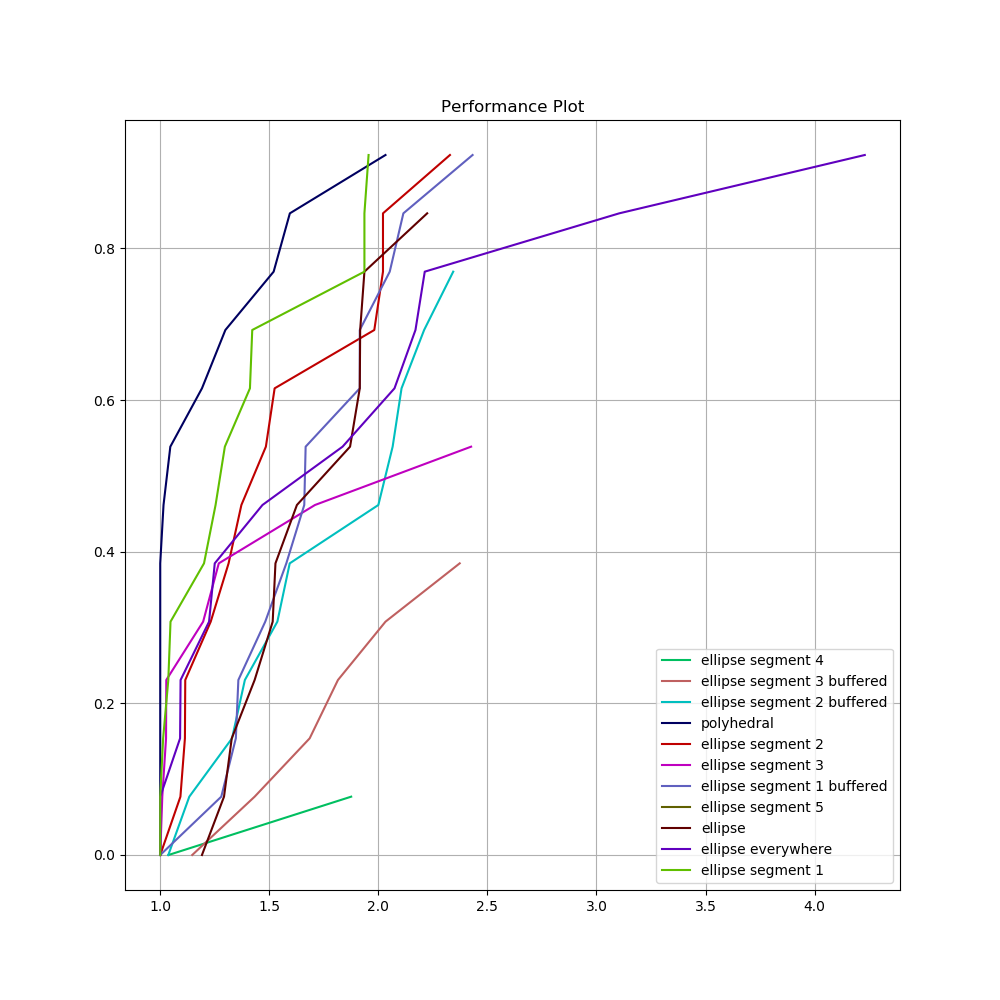
\includegraphics[scale=0.4]{images/performance_profile_plot.png}
    \caption{Performance profile}
    \label{performance_profile}
\end{figure}



The line segment search with 5 segments does not solve many problems, this is because several of the problems have dimension less than $5$, so that it was not even ran on these.
Notice that the polyhedral search does very well.
We conjecture that this may not hold with modelled, nonlinear constraints.


\subsection{Summary}
We still experienced a problem with iterates coming too close to the boundary of the feasible region.
Another way of dealing with this is to shift the constraints closer to the current iterate.
Namely, we introduce a parameter $\upsilon$ to determine how far to scale the constraints.
Then, within the trust region subproblem, we add constraints of $Ax \le b\upsilon + (1-\upsilon) A \xk $.
Before doing this, the rows of $A$ are normalized.
This produces the buffered segment searches withing the results.


\section{Figure out where goes}

\color{red}
From here on, we will assume that the iterates $\xk$ are chosen according to \cref{constrained_dfo}.
This implies that each of the sample points used to construct $\mfk$ are output of \cref{model_improving_algorithm}.

Because \cref{lipschitz_gradient} and \cref{lipschitz_hessian} are satisfied, $f$ also satisfies \cref{introduction_3_1} and hence the assumptions for \cref{quadratic_errors}.
Notice that because $\kappa_f$, $\kappa_g$, $\kappa_h$ only depend on $p$, $L_h$, and $\Lambda$, these values do not depend on the iteration $k$:
using the same tolerance $\xi_{\text{min}}$ within \cref{model_improving_algorithm} implies a bound on $\Lambda$.
, and therefore $\mfk$ satisfies the requirements for \cref{quadratic_errors}.
is a fully quadratic model over $B_{\infty}(\xk, \dk)$.
\color{black}


 

\appendix

\section{Table of Notation}
\begin{longtable}{| p{.20\textwidth} | p{.80\textwidth} |}
$\xk$ & is the current iterate in iteration $k$\\
$\mfk$ & is the model of the objective $f$ during iteration $k$\\
$\mcik$ & is the model of the $i$-th constraint $c_i$ during iteration $k$\\
$\mck$ & is the model of the constraint $c$ during iteration $k$\\
$\dk$ & is the outer trust region radius in iteration $k$ \\
This & is some filler....... \\
$\domain$ & is the domain \\
$\real$ & is the real numbers \\
$f$ & is the objective function \\
$f_{\text{min}}$ & is a lower bound on the objective function \\
$\beta$ & is a bound on the hessian of the model functions \\
$c_i$ & are the constraints $\forall i \in \mathcal{I} \cup \mathcal{E} $ \\
$e_i$ & is the unit vector \\
$\phi_i$ & is a basis vector \\
$Y$ & is the set of sample points \\
$V$ & is a vander mode matrix \\
$y^i$ & is a sample point \\
$d$ & is the dimension of the space of model functions \\
$\lambda_i$ & are the weights of a linear combination \\
$\alpha_i$ & are the coefficients of a model function on its basis polynomials \\
$\phi_i$ & are basis polynomials \\
$p-1$ & is the size of the sample set \\
$l_i$ & is a lagrange polynomial \\
$\Lambda$ & is a constant bounding the poisedness of a sample set \\
$\kappa_{ef},\kappa_{eg},\kappa_{eh}$ & are constants used to bound the model's error \\
$\kappa_{f}$ & is a constant in the efficiency condition \\
$\kappa_{g}$ & is a constant in the accuracy condition \\
$\trialk$ & is the trial point in iteration $k$ \\
$\chik$ & is the criticality measure in iteration $k$ \\
$\outertrk$ & is the outer trust region in iteration $k$ \\
$\feasible$ & is the feasible region \\
$\feasible$ & is the feasible region during iteration $k$ \\
% $\innerfritr$ & is the feasible region intersect the inner trust region \\
$\outerfritr$ & is the feasible region intersect the outer trust region \\
$s$ & is the decision variable within the trust region subproblem \\
$B_k(c; \Delta)$ & is the ball of radius $\Delta$ centered at point $c$ in the $k$ norm\\
& $B_k(c;\Delta) = \{ x \in \mathbb{R}^n : \| x - c\|_k \le \Delta \}$ \\
$\Delta$ & is the trust region radius \\
$\rho$ & measures actual improvement over the predicted improvement \\
$\gamma_1, \gamma_2$ &  are bounds on $\rho$ \\
$\omega_{\text{dec}}, \omega_{\text{inc}}$ & are scalars used to manipulate the trust region radius \\
$\tau$ & is a tolerance \\
$\mathcal{F}^k$ & is the feasible region \\
$f^k$ & is the function value \\
$g^k$ & is the gradient of the model \\
$A$ & is the jacobian of the constraint model functions \\
$\xi_{\text{min}}$ & is a tolerance within the LU pivoting algorithm \\
$T$ & is an affine transformation that brings the trust region back to the origin \\
$Q$ & is the semi-definite matrix defining the affine transformation $T$ \\
$L$ & is a cholesky factorization of $Q$ \\
$L$ & is the Lipschitz constant of $f$ \\
$\mu^k$ & is the center of the ellipse \\
$\ellipsek$ is the ellipse during iteration $k$ \\
$\pi$ & is a scaling factor while finding the ellipse \\
$d$ & are the differences between the center of the ellipse and where the ellipse intersect the constraints? \\
$M$ & is an upper bound \\
$P$ & is a polyhedron \\
$\delta_{i,j}$ & is the kronecker delta function, $\delta_{i,i} = 1$, $\delta_{i,j} = 0$ if $i\ne j$ \\
$\tau_{\xi}$ & is a threshold for the criticallity measure \\
$\tau_{\Delta}$ & is a threshold for the trust region radius
\label{tab:TableOfNotation}
\end{longtable}

\newpage


\bibliography{thesis}
\bibliographystyle{ieeetr}

\end{document}


